\documentclass[11pt,letterpaper]{article}

\usepackage[T1]{fontenc}
\usepackage[utf8]{inputenc}
\usepackage[left=1.0in,right=1.0in,top=1.0in,bottom=1.05in]{geometry}
\usepackage{newpxtext}
\usepackage{newpxmath}
\usepackage[scaled=0.89]{zi4}
\usepackage[protrusion=true,expansion=true]{microtype}

\usepackage{graphicx}
\usepackage{booktabs}
\usepackage{array}
\usepackage{multirow}
\usepackage{enumitem}
\usepackage{xcolor}
\usepackage{tikz}
\usetikzlibrary{arrows.meta,positioning,shapes.geometric}
\usepackage{algorithm}
\usepackage{algpseudocode}
\usepackage[font=small,labelfont=bf,skip=6pt]{caption}
\usepackage[group-separator={,},group-minimum-digits=4]{siunitx}
\usepackage[numbers,sort&compress]{natbib}
\usepackage{hyperref}

\definecolor{oiBlue}{HTML}{0072B2}
\definecolor{oiGreen}{HTML}{009E73}
\definecolor{oiSky}{HTML}{56B4E9}
\definecolor{oiOrange}{HTML}{E69F00}
\definecolor{oiVermilion}{HTML}{D55E00}
\definecolor{oiGray}{HTML}{555555}

\hypersetup{
  colorlinks=true,
  linkcolor=oiBlue,
  citecolor=oiBlue,
  urlcolor=oiBlue,
  pdftitle={Pairwise Valid, Globally Broken: Non-Destructive Lattice Repair and Certification of Multi-Ontology Biological Crosswalk Hubs},
  pdfauthor={[AUTHOR PLACEHOLDER]}
}

\clubpenalty=10000
\widowpenalty=10000
\displaywidowpenalty=10000
\setlength{\parskip}{3pt plus 1pt minus 1pt}
\setlength{\emergencystretch}{1.5em}

\newtheorem{definition}{Definition}
\newtheorem{proposition}{Proposition}

% Programmatic single-source-of-truth empirical macros
% Auto-generated by src/clasp_ont/export/build_figures.py -- DO NOT EDIT MANUALLY
\newcommand{\ClaspTotalClassesAll}{188030}
\newcommand{\ClaspTotalMappingsAll}{41735}
\newcommand{\ClaspMaxPeakRssMBAll}{4289.1}
\newcommand{\ClaspDiseasePhenotypeHubOnts}{5}
\newcommand{\ClaspDiseasePhenotypeHubClasses}{96273}
\newcommand{\ClaspDiseasePhenotypeHubMappings}{24038}
\newcommand{\ClaspDiseasePhenotypeHubRawUnsat}{10644}
\newcommand{\ClaspDiseasePhenotypeHubRawConsViol}{234152}
\newcommand{\ClaspDiseasePhenotypeHubPairwiseUnsat}{6499}
\newcommand{\ClaspDiseasePhenotypeHubPairwiseConsViol}{263119}
\newcommand{\ClaspDiseasePhenotypeHubContestedCount}{20685}
\newcommand{\ClaspDiseasePhenotypeHubInitialCores}{40148}
\newcommand{\ClaspDiseasePhenotypeHubTotalCores}{56116}
\newcommand{\ClaspDiseasePhenotypeHubBFourIters}{16}
\newcommand{\ClaspDiseasePhenotypeHubPeakRssMB}{4289.1}
\newcommand{\ClaspDiseasePhenotypeHubVsBThreeMean}{0.174}
\newcommand{\ClaspDiseasePhenotypeHubVsBThreeLow}{0.169}
\newcommand{\ClaspDiseasePhenotypeHubVsBThreeHigh}{0.180}
\newcommand{\ClaspDiseasePhenotypeHubChapterCount}{586}
\newcommand{\ClaspDiseasePhenotypeHubBRawHubChapterFP}{74475}
\newcommand{\ClaspDiseasePhenotypeHubBRawHubHPMPPairs}{313523}
\newcommand{\ClaspDiseasePhenotypeHubBRawHubDOIDCorruptedPct}{69.1}
\newcommand{\ClaspDiseasePhenotypeHubBRawHubDOIDCorruptedCnt}{10043}
\newcommand{\ClaspDiseasePhenotypeHubBRawHubDOIDJaccard}{0.776}
\newcommand{\ClaspDiseasePhenotypeHubBRawHubHPCorruptedPct}{22.7}
\newcommand{\ClaspDiseasePhenotypeHubBRawHubHPCorruptedCnt}{4649}
\newcommand{\ClaspDiseasePhenotypeHubBRawHubHPJaccard}{0.968}
\newcommand{\ClaspDiseasePhenotypeHubBRawHubMONDOCorruptedPct}{61.3}
\newcommand{\ClaspDiseasePhenotypeHubBRawHubMONDOCorruptedCnt}{21909}
\newcommand{\ClaspDiseasePhenotypeHubBRawHubMONDOJaccard}{0.814}
\newcommand{\ClaspDiseasePhenotypeHubBRawHubMPCorruptedPct}{23.1}
\newcommand{\ClaspDiseasePhenotypeHubBRawHubMPCorruptedCnt}{3560}
\newcommand{\ClaspDiseasePhenotypeHubBRawHubMPJaccard}{0.969}
\newcommand{\ClaspDiseasePhenotypeHubBRawHubORDOCorruptedPct}{85.1}
\newcommand{\ClaspDiseasePhenotypeHubBRawHubORDOCorruptedCnt}{7892}
\newcommand{\ClaspDiseasePhenotypeHubBRawHubORDOJaccard}{0.482}
\newcommand{\ClaspDiseasePhenotypeHubBLogMapRepairChapterFP}{13356}
\newcommand{\ClaspDiseasePhenotypeHubBLogMapRepairHPMPPairs}{302912}
\newcommand{\ClaspDiseasePhenotypeHubBLogMapRepairDOIDCorruptedPct}{34.3}
\newcommand{\ClaspDiseasePhenotypeHubBLogMapRepairDOIDCorruptedCnt}{4989}
\newcommand{\ClaspDiseasePhenotypeHubBLogMapRepairDOIDJaccard}{0.912}
\newcommand{\ClaspDiseasePhenotypeHubBLogMapRepairHPCorruptedPct}{18.1}
\newcommand{\ClaspDiseasePhenotypeHubBLogMapRepairHPCorruptedCnt}{3697}
\newcommand{\ClaspDiseasePhenotypeHubBLogMapRepairHPJaccard}{0.978}
\newcommand{\ClaspDiseasePhenotypeHubBLogMapRepairMONDOCorruptedPct}{0.0}
\newcommand{\ClaspDiseasePhenotypeHubBLogMapRepairMONDOCorruptedCnt}{7}
\newcommand{\ClaspDiseasePhenotypeHubBLogMapRepairMONDOJaccard}{1.000}
\newcommand{\ClaspDiseasePhenotypeHubBLogMapRepairMPCorruptedPct}{6.4}
\newcommand{\ClaspDiseasePhenotypeHubBLogMapRepairMPCorruptedCnt}{987}
\newcommand{\ClaspDiseasePhenotypeHubBLogMapRepairMPJaccard}{0.986}
\newcommand{\ClaspDiseasePhenotypeHubBLogMapRepairORDOCorruptedPct}{3.1}
\newcommand{\ClaspDiseasePhenotypeHubBLogMapRepairORDOCorruptedCnt}{284}
\newcommand{\ClaspDiseasePhenotypeHubBLogMapRepairORDOJaccard}{1.000}
\newcommand{\ClaspDiseasePhenotypeHubBASPBinaryDeleteChapterFP}{0}
\newcommand{\ClaspDiseasePhenotypeHubBASPBinaryDeleteHPMPPairs}{287167}
\newcommand{\ClaspDiseasePhenotypeHubBASPBinaryDeleteDOIDCorruptedPct}{0.0}
\newcommand{\ClaspDiseasePhenotypeHubBASPBinaryDeleteDOIDCorruptedCnt}{0}
\newcommand{\ClaspDiseasePhenotypeHubBASPBinaryDeleteDOIDJaccard}{1.000}
\newcommand{\ClaspDiseasePhenotypeHubBASPBinaryDeleteHPCorruptedPct}{0.0}
\newcommand{\ClaspDiseasePhenotypeHubBASPBinaryDeleteHPCorruptedCnt}{0}
\newcommand{\ClaspDiseasePhenotypeHubBASPBinaryDeleteHPJaccard}{1.000}
\newcommand{\ClaspDiseasePhenotypeHubBASPBinaryDeleteMONDOCorruptedPct}{0.0}
\newcommand{\ClaspDiseasePhenotypeHubBASPBinaryDeleteMONDOCorruptedCnt}{0}
\newcommand{\ClaspDiseasePhenotypeHubBASPBinaryDeleteMONDOJaccard}{1.000}
\newcommand{\ClaspDiseasePhenotypeHubBASPBinaryDeleteMPCorruptedPct}{0.0}
\newcommand{\ClaspDiseasePhenotypeHubBASPBinaryDeleteMPCorruptedCnt}{0}
\newcommand{\ClaspDiseasePhenotypeHubBASPBinaryDeleteMPJaccard}{1.000}
\newcommand{\ClaspDiseasePhenotypeHubBASPBinaryDeleteORDOCorruptedPct}{0.0}
\newcommand{\ClaspDiseasePhenotypeHubBASPBinaryDeleteORDOCorruptedCnt}{0}
\newcommand{\ClaspDiseasePhenotypeHubBASPBinaryDeleteORDOJaccard}{1.000}
\newcommand{\ClaspDiseasePhenotypeHubBLexicalLatticeChapterFP}{0}
\newcommand{\ClaspDiseasePhenotypeHubBLexicalLatticeHPMPPairs}{288767}
\newcommand{\ClaspDiseasePhenotypeHubBLexicalLatticeDOIDCorruptedPct}{0.0}
\newcommand{\ClaspDiseasePhenotypeHubBLexicalLatticeDOIDCorruptedCnt}{0}
\newcommand{\ClaspDiseasePhenotypeHubBLexicalLatticeDOIDJaccard}{1.000}
\newcommand{\ClaspDiseasePhenotypeHubBLexicalLatticeHPCorruptedPct}{0.0}
\newcommand{\ClaspDiseasePhenotypeHubBLexicalLatticeHPCorruptedCnt}{0}
\newcommand{\ClaspDiseasePhenotypeHubBLexicalLatticeHPJaccard}{1.000}
\newcommand{\ClaspDiseasePhenotypeHubBLexicalLatticeMONDOCorruptedPct}{0.0}
\newcommand{\ClaspDiseasePhenotypeHubBLexicalLatticeMONDOCorruptedCnt}{0}
\newcommand{\ClaspDiseasePhenotypeHubBLexicalLatticeMONDOJaccard}{1.000}
\newcommand{\ClaspDiseasePhenotypeHubBLexicalLatticeMPCorruptedPct}{0.0}
\newcommand{\ClaspDiseasePhenotypeHubBLexicalLatticeMPCorruptedCnt}{0}
\newcommand{\ClaspDiseasePhenotypeHubBLexicalLatticeMPJaccard}{1.000}
\newcommand{\ClaspDiseasePhenotypeHubBLexicalLatticeORDOCorruptedPct}{0.0}
\newcommand{\ClaspDiseasePhenotypeHubBLexicalLatticeORDOCorruptedCnt}{0}
\newcommand{\ClaspDiseasePhenotypeHubBLexicalLatticeORDOJaccard}{1.000}
\newcommand{\ClaspDiseasePhenotypeHubBRawHubUnsat}{10644}
\newcommand{\ClaspDiseasePhenotypeHubBRawHubConsViol}{234152}
\newcommand{\ClaspDiseasePhenotypeHubBRawHubRetention}{1.000}
\newcommand{\ClaspDiseasePhenotypeHubBRawHubEquivFone}{0.000}
\newcommand{\ClaspDiseasePhenotypeHubBRawHubSubRecall}{0.000}
\newcommand{\ClaspDiseasePhenotypeHubBRawHubDedSubRecall}{0.000}
\newcommand{\ClaspDiseasePhenotypeHubBRawHubDedSubTP}{0}
\newcommand{\ClaspDiseasePhenotypeHubBRawHubChapterFDRPct}{13.1}
\newcommand{\ClaspDiseasePhenotypeHubBRawHubChapterCross}{559543}
\newcommand{\ClaspDiseasePhenotypeHubBRawHubNovelCross}{1402511}
\newcommand{\ClaspDiseasePhenotypeHubBRawHubKeepEquiv}{24038}
\newcommand{\ClaspDiseasePhenotypeHubBRawHubDowngradeSub}{0}
\newcommand{\ClaspDiseasePhenotypeHubBRawHubDowngradeSup}{0}
\newcommand{\ClaspDiseasePhenotypeHubBRawHubWeakenAncestor}{0}
\newcommand{\ClaspDiseasePhenotypeHubBRawHubDropped}{0}
\newcommand{\ClaspDiseasePhenotypeHubBLogMapRepairUnsat}{1607}
\newcommand{\ClaspDiseasePhenotypeHubBLogMapRepairConsViol}{20045}
\newcommand{\ClaspDiseasePhenotypeHubBLogMapRepairRetention}{0.700}
\newcommand{\ClaspDiseasePhenotypeHubBLogMapRepairEquivFone}{1.000}
\newcommand{\ClaspDiseasePhenotypeHubBLogMapRepairSubRecall}{0.000}
\newcommand{\ClaspDiseasePhenotypeHubBLogMapRepairDedSubRecall}{0.000}
\newcommand{\ClaspDiseasePhenotypeHubBLogMapRepairDedSubTP}{0}
\newcommand{\ClaspDiseasePhenotypeHubBLogMapRepairChapterFDRPct}{2.6}
\newcommand{\ClaspDiseasePhenotypeHubBLogMapRepairChapterCross}{300370}
\newcommand{\ClaspDiseasePhenotypeHubBLogMapRepairNovelCross}{679225}
\newcommand{\ClaspDiseasePhenotypeHubBLogMapRepairKeepEquiv}{22}
\newcommand{\ClaspDiseasePhenotypeHubBLogMapRepairDowngradeSub}{79}
\newcommand{\ClaspDiseasePhenotypeHubBLogMapRepairDowngradeSup}{22302}
\newcommand{\ClaspDiseasePhenotypeHubBLogMapRepairWeakenAncestor}{0}
\newcommand{\ClaspDiseasePhenotypeHubBLogMapRepairDropped}{1635}
\newcommand{\ClaspDiseasePhenotypeHubBASPBinaryDeleteUnsat}{0}
\newcommand{\ClaspDiseasePhenotypeHubBASPBinaryDeleteConsViol}{0}
\newcommand{\ClaspDiseasePhenotypeHubBASPBinaryDeleteRetention}{0.568}
\newcommand{\ClaspDiseasePhenotypeHubBASPBinaryDeleteEquivFone}{0.000}
\newcommand{\ClaspDiseasePhenotypeHubBASPBinaryDeleteSubRecall}{0.000}
\newcommand{\ClaspDiseasePhenotypeHubBASPBinaryDeleteDedSubRecall}{0.000}
\newcommand{\ClaspDiseasePhenotypeHubBASPBinaryDeleteDedSubTP}{0}
\newcommand{\ClaspDiseasePhenotypeHubBASPBinaryDeleteChapterFDRPct}{0.0}
\newcommand{\ClaspDiseasePhenotypeHubBASPBinaryDeleteChapterCross}{345585}
\newcommand{\ClaspDiseasePhenotypeHubBASPBinaryDeleteNovelCross}{767537}
\newcommand{\ClaspDiseasePhenotypeHubBASPBinaryDeleteKeepEquiv}{13659}
\newcommand{\ClaspDiseasePhenotypeHubBASPBinaryDeleteDowngradeSub}{0}
\newcommand{\ClaspDiseasePhenotypeHubBASPBinaryDeleteDowngradeSup}{0}
\newcommand{\ClaspDiseasePhenotypeHubBASPBinaryDeleteWeakenAncestor}{0}
\newcommand{\ClaspDiseasePhenotypeHubBASPBinaryDeleteDropped}{10379}
\newcommand{\ClaspDiseasePhenotypeHubBLexicalLatticeUnsat}{0}
\newcommand{\ClaspDiseasePhenotypeHubBLexicalLatticeConsViol}{0}
\newcommand{\ClaspDiseasePhenotypeHubBLexicalLatticeRetention}{0.735}
\newcommand{\ClaspDiseasePhenotypeHubBLexicalLatticeEquivFone}{0.000}
\newcommand{\ClaspDiseasePhenotypeHubBLexicalLatticeSubRecall}{0.000}
\newcommand{\ClaspDiseasePhenotypeHubBLexicalLatticeDedSubRecall}{0.000}
\newcommand{\ClaspDiseasePhenotypeHubBLexicalLatticeDedSubTP}{0}
\newcommand{\ClaspDiseasePhenotypeHubBLexicalLatticeChapterFDRPct}{0.0}
\newcommand{\ClaspDiseasePhenotypeHubBLexicalLatticeChapterCross}{350785}
\newcommand{\ClaspDiseasePhenotypeHubBLexicalLatticeNovelCross}{816400}
\newcommand{\ClaspDiseasePhenotypeHubBLexicalLatticeKeepEquiv}{6491}
\newcommand{\ClaspDiseasePhenotypeHubBLexicalLatticeDowngradeSub}{11123}
\newcommand{\ClaspDiseasePhenotypeHubBLexicalLatticeDowngradeSup}{3342}
\newcommand{\ClaspDiseasePhenotypeHubBLexicalLatticeWeakenAncestor}{730}
\newcommand{\ClaspDiseasePhenotypeHubBLexicalLatticeDropped}{2352}
\newcommand{\ClaspOAEIBioMLOnts}{4}
\newcommand{\ClaspOAEIBioMLClasses}{43150}
\newcommand{\ClaspOAEIBioMLMappings}{16694}
\newcommand{\ClaspOAEIBioMLRawUnsat}{23619}
\newcommand{\ClaspOAEIBioMLRawConsViol}{33192}
\newcommand{\ClaspOAEIBioMLPairwiseUnsat}{12223}
\newcommand{\ClaspOAEIBioMLPairwiseConsViol}{81821}
\newcommand{\ClaspOAEIBioMLContestedCount}{11537}
\newcommand{\ClaspOAEIBioMLInitialCores}{5753}
\newcommand{\ClaspOAEIBioMLTotalCores}{22564}
\newcommand{\ClaspOAEIBioMLBFourIters}{17}
\newcommand{\ClaspOAEIBioMLPeakRssMB}{3438.1}
\newcommand{\ClaspOAEIBioMLVsBThreeMean}{0.036}
\newcommand{\ClaspOAEIBioMLVsBThreeLow}{0.030}
\newcommand{\ClaspOAEIBioMLVsBThreeHigh}{0.042}
\newcommand{\ClaspOAEIBioMLChapterCount}{220}
\newcommand{\ClaspOAEIBioMLBRawHubChapterFP}{14938}
\newcommand{\ClaspOAEIBioMLBRawHubHPMPPairs}{0}
\newcommand{\ClaspOAEIBioMLBRawHubDOIDCorruptedPct}{80.1}
\newcommand{\ClaspOAEIBioMLBRawHubDOIDCorruptedCnt}{6780}
\newcommand{\ClaspOAEIBioMLBRawHubDOIDJaccard}{0.840}
\newcommand{\ClaspOAEIBioMLBRawHubNCITCorruptedPct}{71.9}
\newcommand{\ClaspOAEIBioMLBRawHubNCITCorruptedCnt}{11326}
\newcommand{\ClaspOAEIBioMLBRawHubNCITJaccard}{0.876}
\newcommand{\ClaspOAEIBioMLBRawHubOMIMCorruptedPct}{44.6}
\newcommand{\ClaspOAEIBioMLBRawHubOMIMCorruptedCnt}{4301}
\newcommand{\ClaspOAEIBioMLBRawHubOMIMJaccard}{0.951}
\newcommand{\ClaspOAEIBioMLBRawHubORDOCorruptedPct}{75.8}
\newcommand{\ClaspOAEIBioMLBRawHubORDOCorruptedCnt}{7027}
\newcommand{\ClaspOAEIBioMLBRawHubORDOJaccard}{0.899}
\newcommand{\ClaspOAEIBioMLBLogMapRepairChapterFP}{2956}
\newcommand{\ClaspOAEIBioMLBLogMapRepairHPMPPairs}{0}
\newcommand{\ClaspOAEIBioMLBLogMapRepairDOIDCorruptedPct}{2.1}
\newcommand{\ClaspOAEIBioMLBLogMapRepairDOIDCorruptedCnt}{176}
\newcommand{\ClaspOAEIBioMLBLogMapRepairDOIDJaccard}{0.995}
\newcommand{\ClaspOAEIBioMLBLogMapRepairNCITCorruptedPct}{7.2}
\newcommand{\ClaspOAEIBioMLBLogMapRepairNCITCorruptedCnt}{1130}
\newcommand{\ClaspOAEIBioMLBLogMapRepairNCITJaccard}{0.989}
\newcommand{\ClaspOAEIBioMLBLogMapRepairOMIMCorruptedPct}{0.0}
\newcommand{\ClaspOAEIBioMLBLogMapRepairOMIMCorruptedCnt}{1}
\newcommand{\ClaspOAEIBioMLBLogMapRepairOMIMJaccard}{1.000}
\newcommand{\ClaspOAEIBioMLBLogMapRepairORDOCorruptedPct}{0.0}
\newcommand{\ClaspOAEIBioMLBLogMapRepairORDOCorruptedCnt}{3}
\newcommand{\ClaspOAEIBioMLBLogMapRepairORDOJaccard}{1.000}
\newcommand{\ClaspOAEIBioMLBASPBinaryDeleteChapterFP}{0}
\newcommand{\ClaspOAEIBioMLBASPBinaryDeleteHPMPPairs}{0}
\newcommand{\ClaspOAEIBioMLBASPBinaryDeleteDOIDCorruptedPct}{0.0}
\newcommand{\ClaspOAEIBioMLBASPBinaryDeleteDOIDCorruptedCnt}{0}
\newcommand{\ClaspOAEIBioMLBASPBinaryDeleteDOIDJaccard}{1.000}
\newcommand{\ClaspOAEIBioMLBASPBinaryDeleteNCITCorruptedPct}{0.0}
\newcommand{\ClaspOAEIBioMLBASPBinaryDeleteNCITCorruptedCnt}{0}
\newcommand{\ClaspOAEIBioMLBASPBinaryDeleteNCITJaccard}{1.000}
\newcommand{\ClaspOAEIBioMLBASPBinaryDeleteOMIMCorruptedPct}{0.0}
\newcommand{\ClaspOAEIBioMLBASPBinaryDeleteOMIMCorruptedCnt}{0}
\newcommand{\ClaspOAEIBioMLBASPBinaryDeleteOMIMJaccard}{1.000}
\newcommand{\ClaspOAEIBioMLBASPBinaryDeleteORDOCorruptedPct}{0.0}
\newcommand{\ClaspOAEIBioMLBASPBinaryDeleteORDOCorruptedCnt}{0}
\newcommand{\ClaspOAEIBioMLBASPBinaryDeleteORDOJaccard}{1.000}
\newcommand{\ClaspOAEIBioMLBLexicalLatticeChapterFP}{0}
\newcommand{\ClaspOAEIBioMLBLexicalLatticeHPMPPairs}{0}
\newcommand{\ClaspOAEIBioMLBLexicalLatticeDOIDCorruptedPct}{0.0}
\newcommand{\ClaspOAEIBioMLBLexicalLatticeDOIDCorruptedCnt}{0}
\newcommand{\ClaspOAEIBioMLBLexicalLatticeDOIDJaccard}{1.000}
\newcommand{\ClaspOAEIBioMLBLexicalLatticeNCITCorruptedPct}{0.0}
\newcommand{\ClaspOAEIBioMLBLexicalLatticeNCITCorruptedCnt}{0}
\newcommand{\ClaspOAEIBioMLBLexicalLatticeNCITJaccard}{1.000}
\newcommand{\ClaspOAEIBioMLBLexicalLatticeOMIMCorruptedPct}{0.0}
\newcommand{\ClaspOAEIBioMLBLexicalLatticeOMIMCorruptedCnt}{0}
\newcommand{\ClaspOAEIBioMLBLexicalLatticeOMIMJaccard}{1.000}
\newcommand{\ClaspOAEIBioMLBLexicalLatticeORDOCorruptedPct}{0.0}
\newcommand{\ClaspOAEIBioMLBLexicalLatticeORDOCorruptedCnt}{0}
\newcommand{\ClaspOAEIBioMLBLexicalLatticeORDOJaccard}{1.000}
\newcommand{\ClaspOAEIBioMLBRawHubUnsat}{23619}
\newcommand{\ClaspOAEIBioMLBRawHubConsViol}{33192}
\newcommand{\ClaspOAEIBioMLBRawHubRetention}{1.000}
\newcommand{\ClaspOAEIBioMLBRawHubEquivFone}{0.648}
\newcommand{\ClaspOAEIBioMLBRawHubSubRecall}{0.000}
\newcommand{\ClaspOAEIBioMLBRawHubDedSubRecall}{0.313}
\newcommand{\ClaspOAEIBioMLBRawHubDedSubTP}{1077}
\newcommand{\ClaspOAEIBioMLBRawHubChapterFDRPct}{21.1}
\newcommand{\ClaspOAEIBioMLBRawHubChapterCross}{60132}
\newcommand{\ClaspOAEIBioMLBRawHubNovelCross}{163895}
\newcommand{\ClaspOAEIBioMLBRawHubKeepEquiv}{16694}
\newcommand{\ClaspOAEIBioMLBRawHubDowngradeSub}{0}
\newcommand{\ClaspOAEIBioMLBRawHubDowngradeSup}{0}
\newcommand{\ClaspOAEIBioMLBRawHubWeakenAncestor}{0}
\newcommand{\ClaspOAEIBioMLBRawHubDropped}{0}
\newcommand{\ClaspOAEIBioMLBLogMapRepairUnsat}{4}
\newcommand{\ClaspOAEIBioMLBLogMapRepairConsViol}{5126}
\newcommand{\ClaspOAEIBioMLBLogMapRepairRetention}{0.749}
\newcommand{\ClaspOAEIBioMLBLogMapRepairEquivFone}{0.009}
\newcommand{\ClaspOAEIBioMLBLogMapRepairSubRecall}{0.000}
\newcommand{\ClaspOAEIBioMLBLogMapRepairDedSubRecall}{0.054}
\newcommand{\ClaspOAEIBioMLBLogMapRepairDedSubTP}{187}
\newcommand{\ClaspOAEIBioMLBLogMapRepairChapterFDRPct}{1.3}
\newcommand{\ClaspOAEIBioMLBLogMapRepairChapterCross}{118518}
\newcommand{\ClaspOAEIBioMLBLogMapRepairNovelCross}{321061}
\newcommand{\ClaspOAEIBioMLBLogMapRepairKeepEquiv}{46}
\newcommand{\ClaspOAEIBioMLBLogMapRepairDowngradeSub}{6185}
\newcommand{\ClaspOAEIBioMLBLogMapRepairDowngradeSup}{10432}
\newcommand{\ClaspOAEIBioMLBLogMapRepairWeakenAncestor}{0}
\newcommand{\ClaspOAEIBioMLBLogMapRepairDropped}{31}
\newcommand{\ClaspOAEIBioMLBASPBinaryDeleteUnsat}{0}
\newcommand{\ClaspOAEIBioMLBASPBinaryDeleteConsViol}{0}
\newcommand{\ClaspOAEIBioMLBASPBinaryDeleteRetention}{0.845}
\newcommand{\ClaspOAEIBioMLBASPBinaryDeleteEquivFone}{0.606}
\newcommand{\ClaspOAEIBioMLBASPBinaryDeleteSubRecall}{0.000}
\newcommand{\ClaspOAEIBioMLBASPBinaryDeleteDedSubRecall}{0.812}
\newcommand{\ClaspOAEIBioMLBASPBinaryDeleteDedSubTP}{2794}
\newcommand{\ClaspOAEIBioMLBASPBinaryDeleteChapterFDRPct}{0.0}
\newcommand{\ClaspOAEIBioMLBASPBinaryDeleteChapterCross}{91931}
\newcommand{\ClaspOAEIBioMLBASPBinaryDeleteNovelCross}{263759}
\newcommand{\ClaspOAEIBioMLBASPBinaryDeleteKeepEquiv}{13962}
\newcommand{\ClaspOAEIBioMLBASPBinaryDeleteDowngradeSub}{0}
\newcommand{\ClaspOAEIBioMLBASPBinaryDeleteDowngradeSup}{0}
\newcommand{\ClaspOAEIBioMLBASPBinaryDeleteWeakenAncestor}{0}
\newcommand{\ClaspOAEIBioMLBASPBinaryDeleteDropped}{2732}
\newcommand{\ClaspOAEIBioMLBLexicalLatticeUnsat}{0}
\newcommand{\ClaspOAEIBioMLBLexicalLatticeConsViol}{0}
\newcommand{\ClaspOAEIBioMLBLexicalLatticeRetention}{0.873}
\newcommand{\ClaspOAEIBioMLBLexicalLatticeEquivFone}{0.663}
\newcommand{\ClaspOAEIBioMLBLexicalLatticeSubRecall}{0.019}
\newcommand{\ClaspOAEIBioMLBLexicalLatticeDedSubRecall}{0.829}
\newcommand{\ClaspOAEIBioMLBLexicalLatticeDedSubTP}{2853}
\newcommand{\ClaspOAEIBioMLBLexicalLatticeChapterFDRPct}{0.0}
\newcommand{\ClaspOAEIBioMLBLexicalLatticeChapterCross}{92476}
\newcommand{\ClaspOAEIBioMLBLexicalLatticeNovelCross}{279461}
\newcommand{\ClaspOAEIBioMLBLexicalLatticeKeepEquiv}{9873}
\newcommand{\ClaspOAEIBioMLBLexicalLatticeDowngradeSub}{3457}
\newcommand{\ClaspOAEIBioMLBLexicalLatticeDowngradeSup}{2535}
\newcommand{\ClaspOAEIBioMLBLexicalLatticeWeakenAncestor}{350}
\newcommand{\ClaspOAEIBioMLBLexicalLatticeDropped}{479}
\newcommand{\ClaspPhaseToyHubOnts}{4}
\newcommand{\ClaspPhaseToyHubClasses}{200}
\newcommand{\ClaspPhaseToyHubMappings}{60}
\newcommand{\ClaspPhaseToyHubRawUnsat}{26}
\newcommand{\ClaspPhaseToyHubRawConsViol}{30}
\newcommand{\ClaspPhaseToyHubPairwiseUnsat}{22}
\newcommand{\ClaspPhaseToyHubPairwiseConsViol}{22}
\newcommand{\ClaspPhaseToyHubContestedCount}{40}
\newcommand{\ClaspPhaseToyHubInitialCores}{34}
\newcommand{\ClaspPhaseToyHubTotalCores}{37}
\newcommand{\ClaspPhaseToyHubBFourIters}{2}
\newcommand{\ClaspPhaseToyHubPeakRssMB}{491.3}
\newcommand{\ClaspPhaseToyHubVsBThreeMean}{0.627}
\newcommand{\ClaspPhaseToyHubVsBThreeLow}{0.502}
\newcommand{\ClaspPhaseToyHubVsBThreeHigh}{0.730}
\newcommand{\ClaspPhaseToyHubChapterCount}{5}
\newcommand{\ClaspPhaseToyHubBRawHubChapterFP}{1}
\newcommand{\ClaspPhaseToyHubBRawHubHPMPPairs}{0}
\newcommand{\ClaspPhaseToyHubBRawHubTOYANATCorruptedPct}{34.0}
\newcommand{\ClaspPhaseToyHubBRawHubTOYANATCorruptedCnt}{17}
\newcommand{\ClaspPhaseToyHubBRawHubTOYANATJaccard}{0.883}
\newcommand{\ClaspPhaseToyHubBRawHubTOYCHEMCorruptedPct}{26.0}
\newcommand{\ClaspPhaseToyHubBRawHubTOYCHEMCorruptedCnt}{13}
\newcommand{\ClaspPhaseToyHubBRawHubTOYCHEMJaccard}{0.936}
\newcommand{\ClaspPhaseToyHubBRawHubTOYPROCCorruptedPct}{22.0}
\newcommand{\ClaspPhaseToyHubBRawHubTOYPROCCorruptedCnt}{11}
\newcommand{\ClaspPhaseToyHubBRawHubTOYPROCJaccard}{0.957}
\newcommand{\ClaspPhaseToyHubBRawHubTOYTRAITCorruptedPct}{18.0}
\newcommand{\ClaspPhaseToyHubBRawHubTOYTRAITCorruptedCnt}{9}
\newcommand{\ClaspPhaseToyHubBRawHubTOYTRAITJaccard}{1.000}
\newcommand{\ClaspPhaseToyHubBLogMapRepairChapterFP}{0}
\newcommand{\ClaspPhaseToyHubBLogMapRepairHPMPPairs}{0}
\newcommand{\ClaspPhaseToyHubBLogMapRepairTOYANATCorruptedPct}{14.0}
\newcommand{\ClaspPhaseToyHubBLogMapRepairTOYANATCorruptedCnt}{7}
\newcommand{\ClaspPhaseToyHubBLogMapRepairTOYANATJaccard}{0.942}
\newcommand{\ClaspPhaseToyHubBLogMapRepairTOYCHEMCorruptedPct}{8.0}
\newcommand{\ClaspPhaseToyHubBLogMapRepairTOYCHEMCorruptedCnt}{4}
\newcommand{\ClaspPhaseToyHubBLogMapRepairTOYCHEMJaccard}{0.969}
\newcommand{\ClaspPhaseToyHubBLogMapRepairTOYPROCCorruptedPct}{10.0}
\newcommand{\ClaspPhaseToyHubBLogMapRepairTOYPROCCorruptedCnt}{5}
\newcommand{\ClaspPhaseToyHubBLogMapRepairTOYPROCJaccard}{0.962}
\newcommand{\ClaspPhaseToyHubBLogMapRepairTOYTRAITCorruptedPct}{0.0}
\newcommand{\ClaspPhaseToyHubBLogMapRepairTOYTRAITCorruptedCnt}{0}
\newcommand{\ClaspPhaseToyHubBLogMapRepairTOYTRAITJaccard}{1.000}
\newcommand{\ClaspPhaseToyHubBASPBinaryDeleteChapterFP}{0}
\newcommand{\ClaspPhaseToyHubBASPBinaryDeleteHPMPPairs}{0}
\newcommand{\ClaspPhaseToyHubBASPBinaryDeleteTOYANATCorruptedPct}{0.0}
\newcommand{\ClaspPhaseToyHubBASPBinaryDeleteTOYANATCorruptedCnt}{0}
\newcommand{\ClaspPhaseToyHubBASPBinaryDeleteTOYANATJaccard}{1.000}
\newcommand{\ClaspPhaseToyHubBASPBinaryDeleteTOYCHEMCorruptedPct}{0.0}
\newcommand{\ClaspPhaseToyHubBASPBinaryDeleteTOYCHEMCorruptedCnt}{0}
\newcommand{\ClaspPhaseToyHubBASPBinaryDeleteTOYCHEMJaccard}{1.000}
\newcommand{\ClaspPhaseToyHubBASPBinaryDeleteTOYPROCCorruptedPct}{0.0}
\newcommand{\ClaspPhaseToyHubBASPBinaryDeleteTOYPROCCorruptedCnt}{0}
\newcommand{\ClaspPhaseToyHubBASPBinaryDeleteTOYPROCJaccard}{1.000}
\newcommand{\ClaspPhaseToyHubBASPBinaryDeleteTOYTRAITCorruptedPct}{0.0}
\newcommand{\ClaspPhaseToyHubBASPBinaryDeleteTOYTRAITCorruptedCnt}{0}
\newcommand{\ClaspPhaseToyHubBASPBinaryDeleteTOYTRAITJaccard}{1.000}
\newcommand{\ClaspPhaseToyHubBLexicalLatticeChapterFP}{0}
\newcommand{\ClaspPhaseToyHubBLexicalLatticeHPMPPairs}{0}
\newcommand{\ClaspPhaseToyHubBLexicalLatticeTOYANATCorruptedPct}{0.0}
\newcommand{\ClaspPhaseToyHubBLexicalLatticeTOYANATCorruptedCnt}{0}
\newcommand{\ClaspPhaseToyHubBLexicalLatticeTOYANATJaccard}{1.000}
\newcommand{\ClaspPhaseToyHubBLexicalLatticeTOYCHEMCorruptedPct}{0.0}
\newcommand{\ClaspPhaseToyHubBLexicalLatticeTOYCHEMCorruptedCnt}{0}
\newcommand{\ClaspPhaseToyHubBLexicalLatticeTOYCHEMJaccard}{1.000}
\newcommand{\ClaspPhaseToyHubBLexicalLatticeTOYPROCCorruptedPct}{0.0}
\newcommand{\ClaspPhaseToyHubBLexicalLatticeTOYPROCCorruptedCnt}{0}
\newcommand{\ClaspPhaseToyHubBLexicalLatticeTOYPROCJaccard}{1.000}
\newcommand{\ClaspPhaseToyHubBLexicalLatticeTOYTRAITCorruptedPct}{0.0}
\newcommand{\ClaspPhaseToyHubBLexicalLatticeTOYTRAITCorruptedCnt}{0}
\newcommand{\ClaspPhaseToyHubBLexicalLatticeTOYTRAITJaccard}{1.000}
\newcommand{\ClaspPhaseToyHubBRawHubUnsat}{26}
\newcommand{\ClaspPhaseToyHubBRawHubConsViol}{30}
\newcommand{\ClaspPhaseToyHubBRawHubRetention}{1.000}
\newcommand{\ClaspPhaseToyHubBRawHubEquivFone}{0.795}
\newcommand{\ClaspPhaseToyHubBRawHubSubRecall}{0.552}
\newcommand{\ClaspPhaseToyHubBRawHubDedSubRecall}{0.276}
\newcommand{\ClaspPhaseToyHubBRawHubDedSubTP}{8}
\newcommand{\ClaspPhaseToyHubBRawHubChapterFDRPct}{1.5}
\newcommand{\ClaspPhaseToyHubBRawHubChapterCross}{170}
\newcommand{\ClaspPhaseToyHubBRawHubNovelCross}{423}
\newcommand{\ClaspPhaseToyHubBRawHubKeepEquiv}{60}
\newcommand{\ClaspPhaseToyHubBRawHubDowngradeSub}{0}
\newcommand{\ClaspPhaseToyHubBRawHubDowngradeSup}{0}
\newcommand{\ClaspPhaseToyHubBRawHubWeakenAncestor}{0}
\newcommand{\ClaspPhaseToyHubBRawHubDropped}{0}
\newcommand{\ClaspPhaseToyHubBLogMapRepairUnsat}{0}
\newcommand{\ClaspPhaseToyHubBLogMapRepairConsViol}{18}
\newcommand{\ClaspPhaseToyHubBLogMapRepairRetention}{0.753}
\newcommand{\ClaspPhaseToyHubBLogMapRepairEquivFone}{0.294}
\newcommand{\ClaspPhaseToyHubBLogMapRepairSubRecall}{0.586}
\newcommand{\ClaspPhaseToyHubBLogMapRepairDedSubRecall}{0.517}
\newcommand{\ClaspPhaseToyHubBLogMapRepairDedSubTP}{15}
\newcommand{\ClaspPhaseToyHubBLogMapRepairChapterFDRPct}{0.0}
\newcommand{\ClaspPhaseToyHubBLogMapRepairChapterCross}{148}
\newcommand{\ClaspPhaseToyHubBLogMapRepairNovelCross}{356}
\newcommand{\ClaspPhaseToyHubBLogMapRepairKeepEquiv}{21}
\newcommand{\ClaspPhaseToyHubBLogMapRepairDowngradeSub}{9}
\newcommand{\ClaspPhaseToyHubBLogMapRepairDowngradeSup}{22}
\newcommand{\ClaspPhaseToyHubBLogMapRepairWeakenAncestor}{0}
\newcommand{\ClaspPhaseToyHubBLogMapRepairDropped}{8}
\newcommand{\ClaspPhaseToyHubBASPBinaryDeleteUnsat}{0}
\newcommand{\ClaspPhaseToyHubBASPBinaryDeleteConsViol}{0}
\newcommand{\ClaspPhaseToyHubBASPBinaryDeleteRetention}{0.774}
\newcommand{\ClaspPhaseToyHubBASPBinaryDeleteEquivFone}{1.000}
\newcommand{\ClaspPhaseToyHubBASPBinaryDeleteSubRecall}{0.552}
\newcommand{\ClaspPhaseToyHubBASPBinaryDeleteDedSubRecall}{0.724}
\newcommand{\ClaspPhaseToyHubBASPBinaryDeleteDedSubTP}{21}
\newcommand{\ClaspPhaseToyHubBASPBinaryDeleteChapterFDRPct}{0.0}
\newcommand{\ClaspPhaseToyHubBASPBinaryDeleteChapterCross}{127}
\newcommand{\ClaspPhaseToyHubBASPBinaryDeleteNovelCross}{318}
\newcommand{\ClaspPhaseToyHubBASPBinaryDeleteKeepEquiv}{45}
\newcommand{\ClaspPhaseToyHubBASPBinaryDeleteDowngradeSub}{0}
\newcommand{\ClaspPhaseToyHubBASPBinaryDeleteDowngradeSup}{0}
\newcommand{\ClaspPhaseToyHubBASPBinaryDeleteWeakenAncestor}{0}
\newcommand{\ClaspPhaseToyHubBASPBinaryDeleteDropped}{15}
\newcommand{\ClaspPhaseToyHubBLexicalLatticeUnsat}{0}
\newcommand{\ClaspPhaseToyHubBLexicalLatticeConsViol}{0}
\newcommand{\ClaspPhaseToyHubBLexicalLatticeRetention}{0.912}
\newcommand{\ClaspPhaseToyHubBLexicalLatticeEquivFone}{0.945}
\newcommand{\ClaspPhaseToyHubBLexicalLatticeSubRecall}{1.000}
\newcommand{\ClaspPhaseToyHubBLexicalLatticeDedSubRecall}{1.000}
\newcommand{\ClaspPhaseToyHubBLexicalLatticeDedSubTP}{29}
\newcommand{\ClaspPhaseToyHubBLexicalLatticeChapterFDRPct}{0.0}
\newcommand{\ClaspPhaseToyHubBLexicalLatticeChapterCross}{132}
\newcommand{\ClaspPhaseToyHubBLexicalLatticeNovelCross}{330}
\newcommand{\ClaspPhaseToyHubBLexicalLatticeKeepEquiv}{42}
\newcommand{\ClaspPhaseToyHubBLexicalLatticeDowngradeSub}{10}
\newcommand{\ClaspPhaseToyHubBLexicalLatticeDowngradeSup}{5}
\newcommand{\ClaspPhaseToyHubBLexicalLatticeWeakenAncestor}{2}
\newcommand{\ClaspPhaseToyHubBLexicalLatticeDropped}{1}
\newcommand{\ClaspPlantBiodivHubOnts}{6}
\newcommand{\ClaspPlantBiodivHubClasses}{48407}
\newcommand{\ClaspPlantBiodivHubMappings}{943}
\newcommand{\ClaspPlantBiodivHubRawUnsat}{40698}
\newcommand{\ClaspPlantBiodivHubRawConsViol}{805}
\newcommand{\ClaspPlantBiodivHubPairwiseUnsat}{18057}
\newcommand{\ClaspPlantBiodivHubPairwiseConsViol}{313763}
\newcommand{\ClaspPlantBiodivHubContestedCount}{887}
\newcommand{\ClaspPlantBiodivHubInitialCores}{68}
\newcommand{\ClaspPlantBiodivHubTotalCores}{2099}
\newcommand{\ClaspPlantBiodivHubBFourIters}{11}
\newcommand{\ClaspPlantBiodivHubPeakRssMB}{2737.4}
\newcommand{\ClaspPlantBiodivHubVsBThreeMean}{0.228}
\newcommand{\ClaspPlantBiodivHubVsBThreeLow}{0.209}
\newcommand{\ClaspPlantBiodivHubVsBThreeHigh}{0.246}
\newcommand{\ClaspPlantBiodivHubChapterCount}{214}
\newcommand{\ClaspPlantBiodivHubBRawHubChapterFP}{0}
\newcommand{\ClaspPlantBiodivHubBRawHubHPMPPairs}{0}
\newcommand{\ClaspPlantBiodivHubBRawHubCHEBICorruptedPct}{88.2}
\newcommand{\ClaspPlantBiodivHubBRawHubCHEBICorruptedCnt}{10356}
\newcommand{\ClaspPlantBiodivHubBRawHubCHEBIJaccard}{1.000}
\newcommand{\ClaspPlantBiodivHubBRawHubENVOCorruptedPct}{22.7}
\newcommand{\ClaspPlantBiodivHubBRawHubENVOCorruptedCnt}{1010}
\newcommand{\ClaspPlantBiodivHubBRawHubENVOJaccard}{1.000}
\newcommand{\ClaspPlantBiodivHubBRawHubFLOPOCorruptedPct}{92.2}
\newcommand{\ClaspPlantBiodivHubBRawHubFLOPOCorruptedCnt}{26193}
\newcommand{\ClaspPlantBiodivHubBRawHubFLOPOJaccard}{0.868}
\newcommand{\ClaspPlantBiodivHubBRawHubGOPLANTCorruptedPct}{57.7}
\newcommand{\ClaspPlantBiodivHubBRawHubGOPLANTCorruptedCnt}{56}
\newcommand{\ClaspPlantBiodivHubBRawHubGOPLANTJaccard}{1.000}
\newcommand{\ClaspPlantBiodivHubBRawHubPOCorruptedPct}{81.8}
\newcommand{\ClaspPlantBiodivHubBRawHubPOCorruptedCnt}{1632}
\newcommand{\ClaspPlantBiodivHubBRawHubPOJaccard}{1.000}
\newcommand{\ClaspPlantBiodivHubBRawHubTOCorruptedPct}{92.3}
\newcommand{\ClaspPlantBiodivHubBRawHubTOCorruptedCnt}{1590}
\newcommand{\ClaspPlantBiodivHubBRawHubTOJaccard}{1.000}
\newcommand{\ClaspPlantBiodivHubBLogMapRepairChapterFP}{1}
\newcommand{\ClaspPlantBiodivHubBLogMapRepairHPMPPairs}{0}
\newcommand{\ClaspPlantBiodivHubBLogMapRepairCHEBICorruptedPct}{88.2}
\newcommand{\ClaspPlantBiodivHubBLogMapRepairCHEBICorruptedCnt}{10350}
\newcommand{\ClaspPlantBiodivHubBLogMapRepairCHEBIJaccard}{1.000}
\newcommand{\ClaspPlantBiodivHubBLogMapRepairENVOCorruptedPct}{21.1}
\newcommand{\ClaspPlantBiodivHubBLogMapRepairENVOCorruptedCnt}{938}
\newcommand{\ClaspPlantBiodivHubBLogMapRepairENVOJaccard}{1.000}
\newcommand{\ClaspPlantBiodivHubBLogMapRepairFLOPOCorruptedPct}{21.1}
\newcommand{\ClaspPlantBiodivHubBLogMapRepairFLOPOCorruptedCnt}{6007}
\newcommand{\ClaspPlantBiodivHubBLogMapRepairFLOPOJaccard}{1.000}
\newcommand{\ClaspPlantBiodivHubBLogMapRepairGOPLANTCorruptedPct}{57.7}
\newcommand{\ClaspPlantBiodivHubBLogMapRepairGOPLANTCorruptedCnt}{56}
\newcommand{\ClaspPlantBiodivHubBLogMapRepairGOPLANTJaccard}{1.000}
\newcommand{\ClaspPlantBiodivHubBLogMapRepairPOCorruptedPct}{0.0}
\newcommand{\ClaspPlantBiodivHubBLogMapRepairPOCorruptedCnt}{0}
\newcommand{\ClaspPlantBiodivHubBLogMapRepairPOJaccard}{1.000}
\newcommand{\ClaspPlantBiodivHubBLogMapRepairTOCorruptedPct}{10.3}
\newcommand{\ClaspPlantBiodivHubBLogMapRepairTOCorruptedCnt}{178}
\newcommand{\ClaspPlantBiodivHubBLogMapRepairTOJaccard}{1.000}
\newcommand{\ClaspPlantBiodivHubBASPBinaryDeleteChapterFP}{0}
\newcommand{\ClaspPlantBiodivHubBASPBinaryDeleteHPMPPairs}{0}
\newcommand{\ClaspPlantBiodivHubBASPBinaryDeleteCHEBICorruptedPct}{0.0}
\newcommand{\ClaspPlantBiodivHubBASPBinaryDeleteCHEBICorruptedCnt}{0}
\newcommand{\ClaspPlantBiodivHubBASPBinaryDeleteCHEBIJaccard}{1.000}
\newcommand{\ClaspPlantBiodivHubBASPBinaryDeleteENVOCorruptedPct}{0.0}
\newcommand{\ClaspPlantBiodivHubBASPBinaryDeleteENVOCorruptedCnt}{0}
\newcommand{\ClaspPlantBiodivHubBASPBinaryDeleteENVOJaccard}{1.000}
\newcommand{\ClaspPlantBiodivHubBASPBinaryDeleteFLOPOCorruptedPct}{0.0}
\newcommand{\ClaspPlantBiodivHubBASPBinaryDeleteFLOPOCorruptedCnt}{0}
\newcommand{\ClaspPlantBiodivHubBASPBinaryDeleteFLOPOJaccard}{1.000}
\newcommand{\ClaspPlantBiodivHubBASPBinaryDeleteGOPLANTCorruptedPct}{0.0}
\newcommand{\ClaspPlantBiodivHubBASPBinaryDeleteGOPLANTCorruptedCnt}{0}
\newcommand{\ClaspPlantBiodivHubBASPBinaryDeleteGOPLANTJaccard}{1.000}
\newcommand{\ClaspPlantBiodivHubBASPBinaryDeletePOCorruptedPct}{0.0}
\newcommand{\ClaspPlantBiodivHubBASPBinaryDeletePOCorruptedCnt}{0}
\newcommand{\ClaspPlantBiodivHubBASPBinaryDeletePOJaccard}{1.000}
\newcommand{\ClaspPlantBiodivHubBASPBinaryDeleteTOCorruptedPct}{0.0}
\newcommand{\ClaspPlantBiodivHubBASPBinaryDeleteTOCorruptedCnt}{0}
\newcommand{\ClaspPlantBiodivHubBASPBinaryDeleteTOJaccard}{1.000}
\newcommand{\ClaspPlantBiodivHubBLexicalLatticeChapterFP}{0}
\newcommand{\ClaspPlantBiodivHubBLexicalLatticeHPMPPairs}{0}
\newcommand{\ClaspPlantBiodivHubBLexicalLatticeCHEBICorruptedPct}{0.0}
\newcommand{\ClaspPlantBiodivHubBLexicalLatticeCHEBICorruptedCnt}{0}
\newcommand{\ClaspPlantBiodivHubBLexicalLatticeCHEBIJaccard}{1.000}
\newcommand{\ClaspPlantBiodivHubBLexicalLatticeENVOCorruptedPct}{0.0}
\newcommand{\ClaspPlantBiodivHubBLexicalLatticeENVOCorruptedCnt}{0}
\newcommand{\ClaspPlantBiodivHubBLexicalLatticeENVOJaccard}{1.000}
\newcommand{\ClaspPlantBiodivHubBLexicalLatticeFLOPOCorruptedPct}{0.0}
\newcommand{\ClaspPlantBiodivHubBLexicalLatticeFLOPOCorruptedCnt}{0}
\newcommand{\ClaspPlantBiodivHubBLexicalLatticeFLOPOJaccard}{1.000}
\newcommand{\ClaspPlantBiodivHubBLexicalLatticeGOPLANTCorruptedPct}{0.0}
\newcommand{\ClaspPlantBiodivHubBLexicalLatticeGOPLANTCorruptedCnt}{0}
\newcommand{\ClaspPlantBiodivHubBLexicalLatticeGOPLANTJaccard}{1.000}
\newcommand{\ClaspPlantBiodivHubBLexicalLatticePOCorruptedPct}{0.0}
\newcommand{\ClaspPlantBiodivHubBLexicalLatticePOCorruptedCnt}{0}
\newcommand{\ClaspPlantBiodivHubBLexicalLatticePOJaccard}{1.000}
\newcommand{\ClaspPlantBiodivHubBLexicalLatticeTOCorruptedPct}{0.0}
\newcommand{\ClaspPlantBiodivHubBLexicalLatticeTOCorruptedCnt}{0}
\newcommand{\ClaspPlantBiodivHubBLexicalLatticeTOJaccard}{1.000}
\newcommand{\ClaspPlantBiodivHubBRawHubUnsat}{40698}
\newcommand{\ClaspPlantBiodivHubBRawHubConsViol}{805}
\newcommand{\ClaspPlantBiodivHubBRawHubRetention}{1.000}
\newcommand{\ClaspPlantBiodivHubBRawHubEquivFone}{0.000}
\newcommand{\ClaspPlantBiodivHubBRawHubSubRecall}{1.000}
\newcommand{\ClaspPlantBiodivHubBRawHubDedSubRecall}{0.000}
\newcommand{\ClaspPlantBiodivHubBRawHubDedSubTP}{0}
\newcommand{\ClaspPlantBiodivHubBRawHubChapterFDRPct}{0.0}
\newcommand{\ClaspPlantBiodivHubBRawHubChapterCross}{138}
\newcommand{\ClaspPlantBiodivHubBRawHubNovelCross}{470}
\newcommand{\ClaspPlantBiodivHubBRawHubKeepEquiv}{943}
\newcommand{\ClaspPlantBiodivHubBRawHubDowngradeSub}{0}
\newcommand{\ClaspPlantBiodivHubBRawHubDowngradeSup}{0}
\newcommand{\ClaspPlantBiodivHubBRawHubWeakenAncestor}{0}
\newcommand{\ClaspPlantBiodivHubBRawHubDropped}{0}
\newcommand{\ClaspPlantBiodivHubBLogMapRepairUnsat}{17518}
\newcommand{\ClaspPlantBiodivHubBLogMapRepairConsViol}{15}
\newcommand{\ClaspPlantBiodivHubBLogMapRepairRetention}{0.739}
\newcommand{\ClaspPlantBiodivHubBLogMapRepairEquivFone}{1.000}
\newcommand{\ClaspPlantBiodivHubBLogMapRepairSubRecall}{0.000}
\newcommand{\ClaspPlantBiodivHubBLogMapRepairDedSubRecall}{0.000}
\newcommand{\ClaspPlantBiodivHubBLogMapRepairDedSubTP}{0}
\newcommand{\ClaspPlantBiodivHubBLogMapRepairChapterFDRPct}{0.0}
\newcommand{\ClaspPlantBiodivHubBLogMapRepairChapterCross}{26349}
\newcommand{\ClaspPlantBiodivHubBLogMapRepairNovelCross}{50542}
\newcommand{\ClaspPlantBiodivHubBLogMapRepairKeepEquiv}{0}
\newcommand{\ClaspPlantBiodivHubBLogMapRepairDowngradeSub}{11}
\newcommand{\ClaspPlantBiodivHubBLogMapRepairDowngradeSup}{920}
\newcommand{\ClaspPlantBiodivHubBLogMapRepairWeakenAncestor}{0}
\newcommand{\ClaspPlantBiodivHubBLogMapRepairDropped}{12}
\newcommand{\ClaspPlantBiodivHubBASPBinaryDeleteUnsat}{0}
\newcommand{\ClaspPlantBiodivHubBASPBinaryDeleteConsViol}{0}
\newcommand{\ClaspPlantBiodivHubBASPBinaryDeleteRetention}{0.243}
\newcommand{\ClaspPlantBiodivHubBASPBinaryDeleteEquivFone}{0.000}
\newcommand{\ClaspPlantBiodivHubBASPBinaryDeleteSubRecall}{1.000}
\newcommand{\ClaspPlantBiodivHubBASPBinaryDeleteDedSubRecall}{0.000}
\newcommand{\ClaspPlantBiodivHubBASPBinaryDeleteDedSubTP}{0}
\newcommand{\ClaspPlantBiodivHubBASPBinaryDeleteChapterFDRPct}{0.0}
\newcommand{\ClaspPlantBiodivHubBASPBinaryDeleteChapterCross}{15428}
\newcommand{\ClaspPlantBiodivHubBASPBinaryDeleteNovelCross}{32979}
\newcommand{\ClaspPlantBiodivHubBASPBinaryDeleteKeepEquiv}{219}
\newcommand{\ClaspPlantBiodivHubBASPBinaryDeleteDowngradeSub}{0}
\newcommand{\ClaspPlantBiodivHubBASPBinaryDeleteDowngradeSup}{0}
\newcommand{\ClaspPlantBiodivHubBASPBinaryDeleteWeakenAncestor}{0}
\newcommand{\ClaspPlantBiodivHubBASPBinaryDeleteDropped}{724}
\newcommand{\ClaspPlantBiodivHubBLexicalLatticeUnsat}{0}
\newcommand{\ClaspPlantBiodivHubBLexicalLatticeConsViol}{0}
\newcommand{\ClaspPlantBiodivHubBLexicalLatticeRetention}{0.532}
\newcommand{\ClaspPlantBiodivHubBLexicalLatticeEquivFone}{0.000}
\newcommand{\ClaspPlantBiodivHubBLexicalLatticeSubRecall}{0.000}
\newcommand{\ClaspPlantBiodivHubBLexicalLatticeDedSubRecall}{0.000}
\newcommand{\ClaspPlantBiodivHubBLexicalLatticeDedSubTP}{0}
\newcommand{\ClaspPlantBiodivHubBLexicalLatticeChapterFDRPct}{0.0}
\newcommand{\ClaspPlantBiodivHubBLexicalLatticeChapterCross}{11026}
\newcommand{\ClaspPlantBiodivHubBLexicalLatticeNovelCross}{26807}
\newcommand{\ClaspPlantBiodivHubBLexicalLatticeKeepEquiv}{175}
\newcommand{\ClaspPlantBiodivHubBLexicalLatticeDowngradeSub}{89}
\newcommand{\ClaspPlantBiodivHubBLexicalLatticeDowngradeSup}{329}
\newcommand{\ClaspPlantBiodivHubBLexicalLatticeWeakenAncestor}{73}
\newcommand{\ClaspPlantBiodivHubBLexicalLatticeDropped}{277}


% Author & institutional placeholders (populate prior to submission)
\newcommand{\ClaspAuthorBlock}{[AUTHOR NAMES PLACEHOLDER]}
\newcommand{\ClaspAffiliationBlock}{[INSTITUTIONAL AFFILIATIONS PLACEHOLDER]}
\newcommand{\ClaspCorrespondenceBlock}{[CORRESPONDING AUTHOR EMAIL PLACEHOLDER]}

\title{\vspace{-1.2em}\textbf{Pairwise Valid, Globally Broken: Non-Destructive Lattice Repair and Certification of Multi-Ontology Biological Crosswalk Hubs}}

\author{\ClaspAuthorBlock\\[0.4em]
\small \ClaspAffiliationBlock\\[0.2em]
\small Correspondence: \texttt{\ClaspCorrespondenceBlock}}

\date{}

\begin{document}
\maketitle
\vspace{-1.0em}

\begin{abstract}
\noindent\textbf{Background:} Genomics, rare-disease, and plant-phenomics platforms routinely merge four to six ontologies through Simple Standard for Sharing Ontological Mappings (SSSOM) crosswalks. Although individual pairs often appear consistent in isolation, composing \texttt{skos:exactMatch} assertions into a unified hub closes cross-ontology cycles and defined-class intersections, rendering valid classes unsatisfiable ($\bot$) and entailing thousands of uncurated intra-ontology subsumptions (conservativity violations). Existing repair tools such as \texttt{LogMap} rely on greedy pairwise deletion, leaving hub-level errors unresolved while discarding valid directional links.

\smallskip
\noindent\textbf{Results:} We present \textsc{CLASP-ONT}, a CPU-only verification and repair engine that optimizes over a five-element subsumption refinement poset ($\equiv$, $\sqsubseteq$, $\sqsupseteq$, ancestor weakening, and negative curation) via two-tier Horn/\textsc{QuickXplain} core extraction and \texttt{Clingo} Counterexample-Guided Abstraction Refinement (CEGAR). Across \num{\ClaspTotalClassesAll} classes and \num{\ClaspTotalMappingsAll} crosswalks in four hubs, composing pairwise mappings inflates unsatisfiable classes by $+93.2\%$ (\num{\ClaspOAEIBioMLPairwiseUnsat} to \num{\ClaspOAEIBioMLRawUnsat}) on \texttt{OAEI\_BioML\_2026}, $+125.4\%$ (\num{\ClaspPlantBiodivHubPairwiseUnsat} to \num{\ClaspPlantBiodivHubRawUnsat}) on \texttt{Plant\_Biodiv\_Hub}, and $+63.8\%$ (\num{\ClaspDiseasePhenotypeHubPairwiseUnsat} to \num{\ClaspDiseasePhenotypeHubRawUnsat}, with \num{\ClaspDiseasePhenotypeHubRawConsViol} conservativity violations) on \texttt{Disease\_Phenotype\_Hub}, where \texttt{LogMap} leaves up to \num{\ClaspDiseasePhenotypeHubBLogMapRepairConsViol} violations unresolved. \textsc{CLASP-ONT} certifies zero post-repair violations across all suites, eliminates $61.7\%\text{--}82.5\%$ of binary hitting-set deletions ($q_{\mathrm{BH}} < 10^{-16}$), and raises \texttt{OAEI\_BioML\_2026} equivalence $F_1$ from \ClaspOAEIBioMLBASPBinaryDeleteEquivFone{} to \ClaspOAEIBioMLBLexicalLatticeEquivFone{} within \ClaspMaxPeakRssMBAll{}~MB RAM.

\smallskip
\noindent\textbf{Conclusions:} Multi-ontology hubs cannot be certified pairwise; \textsc{CLASP-ONT} restores exact coherence and conservativity on a laptop CPU and exports ready-to-merge SSSOM and Knowledge Graph Change Language (KGCL) patches.
\end{abstract}

\vspace{0.3em}
\noindent\small\textbf{Keywords:} Biomedical ontologies; Ontology alignment repair; Deductive conservativity; SSSOM; Knowledge Graph Change Language; Answer Set Programming; OWL~2~EL reasoning
\normalsize

\section*{Background}

Clinical rare-disease diagnostics, translational oncology knowledge graphs, and multi-species plant phenomics all rely on connecting specialized reference ontologies into unified query hubs~\cite{smith2007obofoundry,ashburner2000go}. Rare-disease variant prioritization pipelines merge the Mondo Disease Ontology (\texttt{MONDO}), Human Disease Ontology (\texttt{DOID})~\cite{schriml2012doid}, Orphanet Rare Disease Ontology (\texttt{ORDO}), Human Phenotype Ontology (\texttt{HP})~\cite{gargano2024hpo}, and Mammalian Phenotype Ontology (\texttt{MP}) so that mouse knockout phenotypes can inform human patient diagnosis; plant and ecological trait portals similarly merge the Plant Ontology (\texttt{PO}), Plant Trait Ontology (\texttt{TO}), Flora Phenotype Ontology (\texttt{FLOPO}), Gene Ontology (\texttt{GO}), Chemical Entities of Biological Interest (\texttt{CHEBI}), and Environment Ontology (\texttt{ENVO})~\cite{cooper2018planteome,buttigieg2013envo}. Across these ecosystems, cross-ontology bridges are shared through the Simple Standard for Sharing Ontological Mappings (SSSOM)~\cite{matentzoglu2022sssom} and community repositories such as \texttt{Biomappings}~\cite{hoyt2023biomappings}.

Because automated matchers and legacy database cross-references (\texttt{oboInOwl:hasDbXref}) lack directional calibration, they routinely record asymmetric genus--species relationships as symmetric equivalence (\texttt{skos:exactMatch}, compiled to OWL $s \equiv o$). In live public releases, this conflation corrupts biological meaning in three distinct ways (Fig.~\ref{fig:architecture}A): (i) equating \texttt{DOID:12759} (\emph{choroid cancer}) with \texttt{NCIT:C2949} (\emph{Choroid Neoplasm}) merges malignant ocular carcinomas with benign choroidal neoplasms, contaminating oncology cohort queries; (ii) equating \texttt{PO:0009008} (\emph{plant organ}) with \texttt{ENVO:01000162} (\emph{organ}) collapses botanical structures into taxon-general anatomy; and (iii) equating \texttt{MONDO:0011674} with \texttt{DOID:0110197} imports an anatomical \texttt{RO:0004026} (\emph{disease has location}) existential filler across ontologies, silently forcing \texttt{MONDO:0011674} under the OWL~2~EL defined intersection \texttt{MONDO:0002081} (\emph{musculoskeletal system disorder} $\equiv$ \emph{human disease} $\sqcap \exists\texttt{RO:0004026}.\texttt{UBERON:0002204}$) inside \texttt{MONDO} itself.

Standard ontology release pipelines (such as the OBO Foundry Ontology Development Kit) validate ontologies individually or one pair at a time. Pairwise checks miss multi-hop corruptions because neither ontology alone contains the closing path or disjointness axiom. Once four to six ontologies are composed into a production hub $\mathcal{H}(M)$, two silent failures compromise downstream biological inference:
\begin{enumerate}[leftmargin=1.8em,itemsep=2pt,topsep=3pt]
  \item \textbf{Global logical incoherence ($\mathrm{Unsat}_{\Delta}$):} Crosswalk chains bridge subclasses across native disjointness axioms ($D_1 \sqcap D_2 \sqsubseteq \bot$), collapsing thousands of valid disease, trait, or anatomical classes to \texttt{owl:Nothing}.
  \item \textbf{Deductive conservativity violations ($\mathrm{ConsViol}$):} Even when classes remain satisfiable, composed bridges silently rewrite individual source ontologies by entailing uncurated intra-ontology subsumptions $A \sqsubseteq B$ ($A, B \in \mathrm{Sig}(O_j)$) that distort semantic similarity, gene enrichment, and clinical cohort roll-up~\cite{solimando2017conservativity,antunes2021conservativity}.
\end{enumerate}

Classical alignment repair systems, including \texttt{LogMap}~\cite{jimenezruiz2011logmap} and \texttt{AgreementMakerLight} (\texttt{AML})~\cite{silva2022aml}, operate primarily on ontology pairs and resolve conflicts by deleting offending mappings. Binary deletion treats a recoverable granularity mismatch (\texttt{DOID:12759} $\equiv$ \texttt{NCIT:C2949}) identically to a true homonym (\texttt{PO:0025132} \emph{resin canal} $\equiv$ \texttt{ENVO:00000014} \emph{navigation canal}), severing up to three-quarters of valid cross-species and cross-domain bridges.

\begin{figure}[t]
\centering
\resizebox{0.98\textwidth}{!}{%
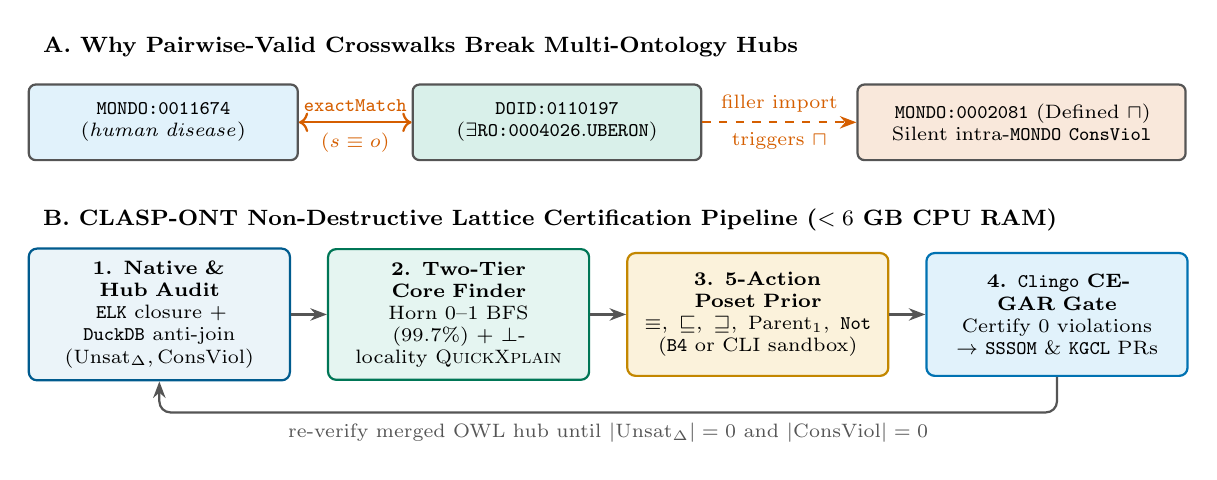
\begin{tikzpicture}[
  font=\scriptsize,
  box/.style={draw=oiGray, rounded corners=2.5pt, thick, align=center, inner sep=4.5pt, minimum height=0.96cm},
  stage/.style={draw=oiBlue!80!black, fill=oiBlue!8, rounded corners=3pt, thick, align=center, minimum height=1.56cm, text width=3.0cm, inner sep=4.5pt},
  arr/.style={-{Stealth[length=2.1mm]}, thick, color=oiGray},
  badarr/.style={-{Stealth[length=2.1mm]}, thick, dashed, color=oiVermilion}
]
  % Panel A header
  \node[anchor=west, font=\footnotesize\bfseries] at (0.05, 2.58) {A. Why Pairwise-Valid Crosswalks Break Multi-Ontology Hubs};
  \node[box, fill=oiSky!18, text width=3.1cm] (m1) at (1.70, 1.62) {\texttt{MONDO:0011674}\\(\emph{human disease})};
  \node[box, fill=oiGreen!15, text width=3.35cm] (d1) at (6.70, 1.62) {\texttt{DOID:0110197}\\($\exists\texttt{RO:0004026}.\texttt{UBERON}$)};
  \node[box, fill=oiVermilion!14, text width=3.85cm] (m2) at (12.60, 1.62) {\texttt{MONDO:0002081} (Defined $\sqcap$)\\Silent intra-\texttt{MONDO} \texttt{ConsViol}};

  \draw[arr, <->, color=oiVermilion, thick] (m1) -- node[above, font=\scriptsize] {\texttt{exactMatch}} node[below, font=\scriptsize, color=oiVermilion] {($s \equiv o$)} (d1);
  \draw[badarr] (d1) -- node[above, font=\scriptsize, color=oiVermilion] {filler import} node[below, font=\scriptsize, color=oiVermilion] {triggers $\sqcap$} (m2);

  % Panel B header
  \node[anchor=west, font=\footnotesize\bfseries] at (0.05, 0.38) {B. \textsc{CLASP-ONT} Non-Destructive Lattice Certification Pipeline ($<6$~GB CPU RAM)};
  \node[stage] (s1) at (1.65, -0.82) {\textbf{1. Native \& Hub Audit}\\\texttt{ELK} closure + \texttt{DuckDB} anti-join ($\mathrm{Unsat}_{\Delta}, \mathrm{ConsViol}$)};
  \node[stage, fill=oiGreen!10, draw=oiGreen!75!black] (s2) at (5.45, -0.82) {\textbf{2. Two-Tier Core Finder}\\Horn $0\text{--}1$ BFS ($99.7\%$) + $\bot$-locality \textsc{QuickXplain}};
  \node[stage, fill=oiOrange!14, draw=oiOrange!85!black] (s3) at (9.25, -0.82) {\textbf{3. 5-Action Poset Prior}\\$\equiv,\; \sqsubseteq,\; \sqsupseteq,\; \mathrm{Parent}_1,\; \texttt{Not}$ (\texttt{B4} or CLI sandbox)};
  \node[stage, fill=oiSky!18, draw=oiBlue] (s4) at (13.05, -0.82) {\textbf{4. \texttt{Clingo} CEGAR Gate}\\Certify $0$ violations $\to$ \texttt{SSSOM} \& \texttt{KGCL} PRs};

  \draw[arr] (s1) -- (s2);
  \draw[arr] (s2) -- (s3);
  \draw[arr] (s3) -- (s4);
  \draw[arr, rounded corners=4pt] (s4.south) -- ++(0,-0.45) -| node[pos=0.25, below, font=\scriptsize] {re-verify merged OWL hub until $|\mathrm{Unsat}_{\Delta}| = 0$ and $|\mathrm{ConsViol}| = 0$} (s1.south);
\end{tikzpicture}%
}
\caption{\textbf{Problem mechanism and \textsc{CLASP-ONT} architecture.} \textbf{A.} Asserting symmetric equivalence ($\equiv$) across ontologies transfers existential fillers that trigger unintended OWL~2~EL defined-class classifications inside a single source ontology ($\mathrm{ConsViol}$) or cross-kingdom disjointness crashes ($\mathrm{Unsat}_{\Delta}$). \textbf{B.} Four-stage symbolic certification and refinement pipeline guaranteeing exact zero hub violations while refining contested equivalences into directional subsumptions.}
\label{fig:architecture}
\end{figure}

Following Medvedev's classification for algorithmic bioinformatics contributions~\cite{medvedev2023theoretical}, we state our three contributions explicitly and separate classical components from new methods (Fig.~\ref{fig:architecture}B). First, at the \emph{problem formulation} level, we cast multi-ontology hub certification as maximum-utility optimization over a five-element subsumption refinement poset $\mathcal{L}(m_i)$ subject to exact zero-unsatisfiability and zero-conservativity invariants across all $k$ constituent ontologies simultaneously. Second, at the \emph{algorithmic} level, whereas \texttt{ELK} polynomial saturation~\cite{kazakov2014elk}, $\bot$-locality modules~\cite{cuencagrau2008modular}, and \texttt{Clingo} Answer Set Programming (ASP)~\cite{gebser2011potassco,gebser2019clingo} are established building blocks, we introduce a two-tier minimal conflict core extractor that augments native hierarchies with conservative anonymous intersection witnesses (\texttt{urn:clasp:anon:*}) for conjunctive Horn $0\text{--}1$ breadth-first search (BFS), resolving $>99.7\%$ of defined-class existential violations in memory before invoking indexed $\bot$-locality \textsc{QuickXplain} and Counterexample-Guided Abstraction Refinement (CEGAR)~\cite{clarke2003cegar}. Third, at the \emph{software and community} level, we release \textsc{CLASP-ONT}, a reproducible CPU-only toolkit ($< 6$~GB RAM, zero GPU or local language-model weights) that serves ontology curators, clinical knowledge-graph engineers, and plant/disease database maintainers by exporting certified SSSOM crosswalks and ready-to-merge Knowledge Graph Change Language (KGCL) pull-request patches.

\section*{Results}

\subsection*{Pairwise-valid crosswalks fracture in multi-ontology hubs}

To test whether pairwise alignment checks suffice for multi-ontology integration (Hypothesis~H1), we audited four benchmark suites spanning \num{\ClaspTotalClassesAll} classes and \num{\ClaspTotalMappingsAll} crosswalks (Table~\ref{tab:h1_breakdown}; Fig.~\ref{fig:compositional}): a deterministic 4-ontology synthetic control with planted diamond and disjointness traps (\texttt{Phase0\_Toy\_Hub}, \num{\ClaspPhaseToyHubClasses} classes, \num{\ClaspPhaseToyHubMappings} mappings), the 4-ontology oncology and rare-disease suite with held-out equivalence and directional subsumption reference sets (\texttt{OAEI\_BioML\_2026}~\cite{he2022bioml}, \num{\ClaspOAEIBioMLClasses} classes, \num{\ClaspOAEIBioMLMappings} mappings), a 6-ontology plant and environmental hub (\texttt{Plant\_Biodiv\_Hub}, \num{\ClaspPlantBiodivHubClasses} classes, \num{\ClaspPlantBiodivHubMappings} mappings), and a 5-ontology clinical and mammalian phenotype hub (\texttt{Disease\_Phenotype\_Hub}, \num{\ClaspDiseasePhenotypeHubClasses} classes, \num{\ClaspDiseasePhenotypeHubMappings} mappings). Prior to evaluating crosswalks, Stage~1 isolated all pre-existing native unsatisfiable classes and embedded cross-namespace axioms in the unmapped union $\mathcal{H}(\emptyset) = O_1 \cup \dots \cup O_k$ so that $\mathrm{Unsat}_{\Delta}$ and $\mathrm{ConsViol}$ measure strictly alignment-induced defects.

\begin{table}[t]
\centering
\caption{\textbf{Compositional breakdown across multi-ontology hubs (Hypothesis~H1).} Summing independent pairwise audits $(O_i, O_j)$ undercounts hub-emergent unsatisfiable classes ($\mathrm{Unsat}_{\Delta}$) by $38.9\%$ to $55.6\%$ across all three public hubs. Note that summed pairwise $\mathrm{ConsViol}$ can exceed merged $\mathrm{ConsViol}$ when classes entailed as satisfiable subclasses pairwise collapse to $\bot$ in the full hub and transfer into $\mathrm{Unsat}_{\Delta}$.}
\label{tab:h1_breakdown}
\small
\setlength{\tabcolsep}{4.8pt}
\begin{tabular}{@{}lrrrrrrr@{}}
\toprule
& & & & \multicolumn{2}{c}{\textbf{Summed Pairwise}} & \multicolumn{2}{c}{\textbf{Merged Hub (\texttt{B1})}} \\
\cmidrule(lr){5-6}\cmidrule(l){7-8}
\textbf{Evaluation Suite} & \textbf{Onts} & \textbf{Classes} & \textbf{Mappings} & $\sum \mathrm{Unsat}$ & $\sum \mathrm{ConsViol}$ & $|\mathrm{Unsat}_{\Delta}|$ & $|\mathrm{ConsViol}|$ \\
\midrule
\texttt{Phase0\_Toy\_Hub} & \ClaspPhaseToyHubOnts{} & \num{\ClaspPhaseToyHubClasses} & \num{\ClaspPhaseToyHubMappings} & \num{\ClaspPhaseToyHubPairwiseUnsat} & \num{\ClaspPhaseToyHubPairwiseConsViol} & \textbf{\num{\ClaspPhaseToyHubRawUnsat}} & \textbf{\num{\ClaspPhaseToyHubRawConsViol}} \\
\texttt{OAEI\_BioML\_2026} & \ClaspOAEIBioMLOnts{} & \num{\ClaspOAEIBioMLClasses} & \num{\ClaspOAEIBioMLMappings} & \num{\ClaspOAEIBioMLPairwiseUnsat} & \num{\ClaspOAEIBioMLPairwiseConsViol} & \textbf{\num{\ClaspOAEIBioMLRawUnsat}} & \textbf{\num{\ClaspOAEIBioMLRawConsViol}} \\
\texttt{Plant\_Biodiv\_Hub} & \ClaspPlantBiodivHubOnts{} & \num{\ClaspPlantBiodivHubClasses} & \num{\ClaspPlantBiodivHubMappings} & \num{\ClaspPlantBiodivHubPairwiseUnsat} & \num{\ClaspPlantBiodivHubPairwiseConsViol} & \textbf{\num{\ClaspPlantBiodivHubRawUnsat}} & \textbf{\num{\ClaspPlantBiodivHubRawConsViol}} \\
\texttt{Disease\_Phenotype\_Hub} & \ClaspDiseasePhenotypeHubOnts{} & \num{\ClaspDiseasePhenotypeHubClasses} & \num{\ClaspDiseasePhenotypeHubMappings} & \num{\ClaspDiseasePhenotypeHubPairwiseUnsat} & \num{\ClaspDiseasePhenotypeHubPairwiseConsViol} & \textbf{\num{\ClaspDiseasePhenotypeHubRawUnsat}} & \textbf{\num{\ClaspDiseasePhenotypeHubRawConsViol}} \\
\bottomrule
\end{tabular}
\end{table}

\begin{figure}[t]
\centering
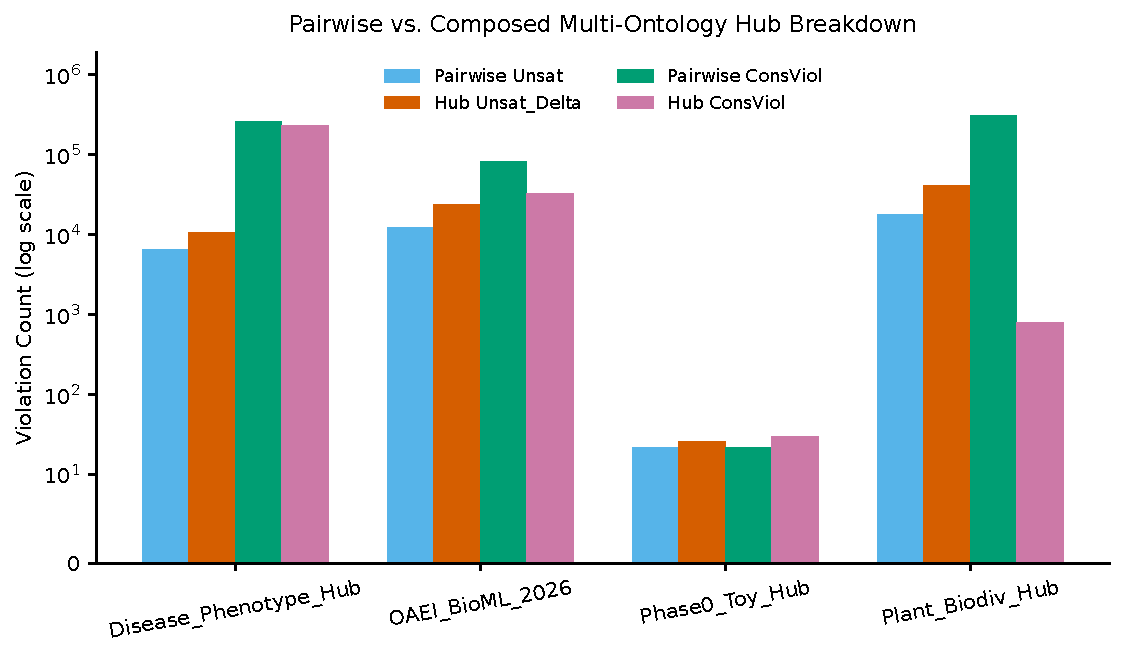
\includegraphics[width=0.88\textwidth]{../results/figures/fig1_compositional_breakdown.pdf}
\caption{\textbf{Pairwise versus composed multi-ontology hub defects.} Log-scaled counts of alignment-induced unsatisfiable classes ($\mathrm{Unsat}_{\Delta}$) and intra-ontology conservativity violations ($\mathrm{ConsViol}$) when evaluating ontology pairs independently versus merging all $k$ ontologies simultaneously.}
\label{fig:compositional}
\end{figure}

Across every public suite, pairwise auditing missed the majority of global unsatisfiability cascades (Table~\ref{tab:h1_breakdown}). On \texttt{OAEI\_BioML\_2026}, four of the six ontology pairs exhibited zero pairwise unsatisfiable classes in isolation, yet composing all four ontologies nearly doubled $\mathrm{Unsat}_{\Delta}$ from \num{\ClaspOAEIBioMLPairwiseUnsat} to \num{\ClaspOAEIBioMLRawUnsat} ($+93.2\%$) alongside \num{\ClaspOAEIBioMLRawConsViol} conservativity violations. On \texttt{Plant\_Biodiv\_Hub}, merging six botanical, biochemical, and environmental ontologies increased $\mathrm{Unsat}_{\Delta}$ by $+125.4\%$ (\num{\ClaspPlantBiodivHubPairwiseUnsat} pairwise to \num{\ClaspPlantBiodivHubRawUnsat} in the full hub), collapsing $84.1\%$ of satisfiable hub classes into $\bot$ via high-level BFO/ENVO/PO disjointness axioms; this collapse simultaneously explains why pairwise $\mathrm{ConsViol}$ rows (\num{\ClaspPlantBiodivHubPairwiseConsViol}) converted into full-hub unsatisfiabilities rather than satisfiable subsumptions (\num{\ClaspPlantBiodivHubRawConsViol}). On \texttt{Disease\_Phenotype\_Hub}, full composition produced \num{\ClaspDiseasePhenotypeHubRawUnsat} alignment-induced unsatisfiable classes ($+63.8\%$ above the pairwise sum of \num{\ClaspDiseasePhenotypeHubPairwiseUnsat}) and \num{\ClaspDiseasePhenotypeHubRawConsViol} intra-ontology conservativity violations, driven heavily by OWL~2~EL defined-class intersections (\texttt{IntersectionOf} with \texttt{RO} and \texttt{UBERON}/\texttt{HP} existential fillers) across \texttt{MONDO}, \texttt{DOID}, \texttt{HP}, and \texttt{MP}.

\subsection*{Greedy pairwise repair leaves hub violations unresolved and degrades $F_1$}

We first evaluated whether standalone \texttt{LogMap~4.0} repair (\texttt{B2\_LogMap\_Repair}), applied across every ontology pair and re-evaluated in the merged hub, can restore coherence and conservativity (Table~\ref{tab:main_benchmark}). On all four suites, \texttt{B2\_LogMap\_Repair} failed the mathematical certification gate ($|\mathrm{Unsat}_{\Delta}| = 0$ and $|\mathrm{ConsViol}| = 0$). On \texttt{OAEI\_BioML\_2026}, \texttt{LogMap} reduced $\mathrm{Unsat}_{\Delta}$ to \num{\ClaspOAEIBioMLBLogMapRepairUnsat} but left \num{\ClaspOAEIBioMLBLogMapRepairConsViol} intra-ontology conservativity violations intact; worse, its uncalibrated pairwise orientation rewrote \num{\ClaspOAEIBioMLBLogMapRepairDowngradeSub} mappings to $\sqsubseteq$ and \num{\ClaspOAEIBioMLBLogMapRepairDowngradeSup} to $\sqsupseteq$, retaining only \num{\ClaspOAEIBioMLBLogMapRepairKeepEquiv} equivalences and collapsing held-out equivalence $F_1$ from \ClaspOAEIBioMLBRawHubEquivFone{} (\texttt{B1}) to \ClaspOAEIBioMLBLogMapRepairEquivFone{}. On \texttt{Plant\_Biodiv\_Hub} and \texttt{Disease\_Phenotype\_Hub}, \texttt{B2\_LogMap\_Repair} left \num{\ClaspPlantBiodivHubBLogMapRepairUnsat} and \num{\ClaspDiseasePhenotypeHubBLogMapRepairUnsat} unsatisfiable classes, plus \num{\ClaspPlantBiodivHubBLogMapRepairConsViol} and \num{\ClaspDiseasePhenotypeHubBLogMapRepairConsViol} conservativity violations, respectively.

\begin{table}[t]
\centering
\caption{\textbf{Multi-ontology hub repair, certification, and semantic retention across all four suites.} \texttt{B3\_ASP\_Binary\_Delete} restricts \texttt{Clingo} CEGAR to binary $\{\text{keep}, \text{drop}\}$; \texttt{B4\_Lexical\_Lattice} (\textsc{CLASP-ONT} with deterministic TF-IDF/hierarchy priors) optimizes over all five refinement poset actions. Every \texttt{B3} and \texttt{B4} output is independently verified to satisfy $|\mathrm{Unsat}_{\Delta}| = 0$ and $|\mathrm{ConsViol}| = 0$. Note: on \texttt{Plant\_Biodiv\_Hub} and \texttt{Disease\_Phenotype\_Hub}, no external held-out gold alignment file exists, so benchmark $F_1$ is evaluated on \texttt{OAEI\_BioML\_2026} and \texttt{Phase0\_Toy\_Hub}.}
\label{tab:main_benchmark}
\footnotesize
\setlength{\tabcolsep}{3.6pt}
\resizebox{\textwidth}{!}{%
\begin{tabular}{@{}llrrrrrrr@{}}
\toprule
\textbf{Suite} & \textbf{System} & $|\mathrm{Unsat}_{\Delta}|$ & $|\mathrm{ConsViol}|$ & \textbf{Keep $\equiv$} & \textbf{Refined} & \textbf{Dropped} & \textbf{Equiv $F_1$} & \textbf{Retention} \\
\midrule
\multirow{4}{*}{\texttt{OAEI\_BioML\_2026}}
 & \texttt{B1\_Raw\_Hub} & \num{\ClaspOAEIBioMLBRawHubUnsat} & \num{\ClaspOAEIBioMLBRawHubConsViol} & \num{\ClaspOAEIBioMLBRawHubKeepEquiv} & 0 & \num{\ClaspOAEIBioMLBRawHubDropped} & \ClaspOAEIBioMLBRawHubEquivFone{} & \ClaspOAEIBioMLBRawHubRetention{} \\
 & \texttt{B2\_LogMap\_Repair} & \num{\ClaspOAEIBioMLBLogMapRepairUnsat} & \num{\ClaspOAEIBioMLBLogMapRepairConsViol} & \num{\ClaspOAEIBioMLBLogMapRepairKeepEquiv} & \num{16617} & \num{\ClaspOAEIBioMLBLogMapRepairDropped} & \ClaspOAEIBioMLBLogMapRepairEquivFone{} & \ClaspOAEIBioMLBLogMapRepairRetention{} \\
 & \texttt{B3\_ASP\_Binary\_Delete} & \textbf{\num{\ClaspOAEIBioMLBASPBinaryDeleteUnsat}} & \textbf{\num{\ClaspOAEIBioMLBASPBinaryDeleteConsViol}} & \num{\ClaspOAEIBioMLBASPBinaryDeleteKeepEquiv} & 0 & \num{\ClaspOAEIBioMLBASPBinaryDeleteDropped} & \ClaspOAEIBioMLBASPBinaryDeleteEquivFone{} & \ClaspOAEIBioMLBASPBinaryDeleteRetention{} \\
 & \texttt{B4\_Lexical\_Lattice} & \textbf{\num{\ClaspOAEIBioMLBLexicalLatticeUnsat}} & \textbf{\num{\ClaspOAEIBioMLBLexicalLatticeConsViol}} & \num{\ClaspOAEIBioMLBLexicalLatticeKeepEquiv} & \num{6342} & \textbf{\num{\ClaspOAEIBioMLBLexicalLatticeDropped}} & \textbf{\ClaspOAEIBioMLBLexicalLatticeEquivFone{}} & \textbf{\ClaspOAEIBioMLBLexicalLatticeRetention{}} \\
\addlinespace[3pt]
\multirow{4}{*}{\texttt{Plant\_Biodiv\_Hub}}
 & \texttt{B1\_Raw\_Hub} & \num{\ClaspPlantBiodivHubBRawHubUnsat} & \num{\ClaspPlantBiodivHubBRawHubConsViol} & \num{\ClaspPlantBiodivHubBRawHubKeepEquiv} & 0 & \num{\ClaspPlantBiodivHubBRawHubDropped} & --- & \ClaspPlantBiodivHubBRawHubRetention{} \\
 & \texttt{B2\_LogMap\_Repair} & \num{\ClaspPlantBiodivHubBLogMapRepairUnsat} & \num{\ClaspPlantBiodivHubBLogMapRepairConsViol} & \num{\ClaspPlantBiodivHubBLogMapRepairKeepEquiv} & 931 & \num{\ClaspPlantBiodivHubBLogMapRepairDropped} & --- & \ClaspPlantBiodivHubBLogMapRepairRetention{} \\
 & \texttt{B3\_ASP\_Binary\_Delete} & \textbf{\num{\ClaspPlantBiodivHubBASPBinaryDeleteUnsat}} & \textbf{\num{\ClaspPlantBiodivHubBASPBinaryDeleteConsViol}} & \num{\ClaspPlantBiodivHubBASPBinaryDeleteKeepEquiv} & 0 & \num{\ClaspPlantBiodivHubBASPBinaryDeleteDropped} & --- & \ClaspPlantBiodivHubBASPBinaryDeleteRetention{} \\
 & \texttt{B4\_Lexical\_Lattice} & \textbf{\num{\ClaspPlantBiodivHubBLexicalLatticeUnsat}} & \textbf{\num{\ClaspPlantBiodivHubBLexicalLatticeConsViol}} & \num{\ClaspPlantBiodivHubBLexicalLatticeKeepEquiv} & 491 & \textbf{\num{\ClaspPlantBiodivHubBLexicalLatticeDropped}} & --- & \textbf{\ClaspPlantBiodivHubBLexicalLatticeRetention{}} \\
\addlinespace[3pt]
\multirow{4}{*}{\texttt{Disease\_Phenotype\_Hub}}
 & \texttt{B1\_Raw\_Hub} & \num{\ClaspDiseasePhenotypeHubBRawHubUnsat} & \num{\ClaspDiseasePhenotypeHubBRawHubConsViol} & \num{\ClaspDiseasePhenotypeHubBRawHubKeepEquiv} & 0 & \num{\ClaspDiseasePhenotypeHubBRawHubDropped} & --- & \ClaspDiseasePhenotypeHubBRawHubRetention{} \\
 & \texttt{B2\_LogMap\_Repair} & \num{\ClaspDiseasePhenotypeHubBLogMapRepairUnsat} & \num{\ClaspDiseasePhenotypeHubBLogMapRepairConsViol} & \num{\ClaspDiseasePhenotypeHubBLogMapRepairKeepEquiv} & \num{22381} & \num{\ClaspDiseasePhenotypeHubBLogMapRepairDropped} & --- & \ClaspDiseasePhenotypeHubBLogMapRepairRetention{} \\
 & \texttt{B3\_ASP\_Binary\_Delete} & \textbf{\num{\ClaspDiseasePhenotypeHubBASPBinaryDeleteUnsat}} & \textbf{\num{\ClaspDiseasePhenotypeHubBASPBinaryDeleteConsViol}} & \num{\ClaspDiseasePhenotypeHubBASPBinaryDeleteKeepEquiv} & 0 & \num{\ClaspDiseasePhenotypeHubBASPBinaryDeleteDropped} & --- & \ClaspDiseasePhenotypeHubBASPBinaryDeleteRetention{} \\
 & \texttt{B4\_Lexical\_Lattice} & \textbf{\num{\ClaspDiseasePhenotypeHubBLexicalLatticeUnsat}} & \textbf{\num{\ClaspDiseasePhenotypeHubBLexicalLatticeConsViol}} & \num{\ClaspDiseasePhenotypeHubBLexicalLatticeKeepEquiv} & \num{15195} & \textbf{\num{\ClaspDiseasePhenotypeHubBLexicalLatticeDropped}} & --- & \textbf{\ClaspDiseasePhenotypeHubBLexicalLatticeRetention{}} \\
\addlinespace[3pt]
\multirow{4}{*}{\texttt{Phase0\_Toy\_Hub}}
 & \texttt{B1\_Raw\_Hub} & \num{\ClaspPhaseToyHubBRawHubUnsat} & \num{\ClaspPhaseToyHubBRawHubConsViol} & \num{\ClaspPhaseToyHubBRawHubKeepEquiv} & 0 & \num{\ClaspPhaseToyHubBRawHubDropped} & \ClaspPhaseToyHubBRawHubEquivFone{} & \ClaspPhaseToyHubBRawHubRetention{} \\
 & \texttt{B2\_LogMap\_Repair} & \num{\ClaspPhaseToyHubBLogMapRepairUnsat} & \num{\ClaspPhaseToyHubBLogMapRepairConsViol} & \num{\ClaspPhaseToyHubBLogMapRepairKeepEquiv} & 31 & \num{\ClaspPhaseToyHubBLogMapRepairDropped} & \ClaspPhaseToyHubBLogMapRepairEquivFone{} & \ClaspPhaseToyHubBLogMapRepairRetention{} \\
 & \texttt{B3\_ASP\_Binary\_Delete} & \textbf{\num{\ClaspPhaseToyHubBASPBinaryDeleteUnsat}} & \textbf{\num{\ClaspPhaseToyHubBASPBinaryDeleteConsViol}} & \num{\ClaspPhaseToyHubBASPBinaryDeleteKeepEquiv} & 0 & \num{\ClaspPhaseToyHubBASPBinaryDeleteDropped} & \textbf{\ClaspPhaseToyHubBASPBinaryDeleteEquivFone{}} & \ClaspPhaseToyHubBASPBinaryDeleteRetention{} \\
 & \texttt{B4\_Lexical\_Lattice} & \textbf{\num{\ClaspPhaseToyHubBLexicalLatticeUnsat}} & \textbf{\num{\ClaspPhaseToyHubBLexicalLatticeConsViol}} & \num{\ClaspPhaseToyHubBLexicalLatticeKeepEquiv} & 17 & \textbf{\num{\ClaspPhaseToyHubBLexicalLatticeDropped}} & \ClaspPhaseToyHubBLexicalLatticeEquivFone{} & \textbf{\ClaspPhaseToyHubBLexicalLatticeRetention{}} \\
\bottomrule
\end{tabular}%
}
\end{table}

\subsection*{Five-action lattice CEGAR eliminates $62\%\text{--}83\%$ of deletions at zero violations}

To isolate the exact contribution of the five-element subsumption refinement poset over optimal axiom deletion (Hypothesis~H2), we conducted a controlled lattice-space ablation comparing \texttt{B3\_ASP\_Binary\_Delete} (an ablation of \textsc{CLASP-ONT} restricting the identical \texttt{Clingo} CEGAR loop to binary $\{\texttt{keep\_equiv}, \texttt{negate\_drop}\}$) against \texttt{B4\_Lexical\_Lattice}, which unlocks directional subsumption ($\sqsubseteq$, $\sqsupseteq$) and single-step ancestor weakening scored by deterministic TF-IDF definition similarity and ontology tree depth (Table~\ref{tab:main_benchmark}; Figs.~\ref{fig:bioml_acc} and~\ref{fig:lattice_fates}).

\begin{figure}[t]
\centering
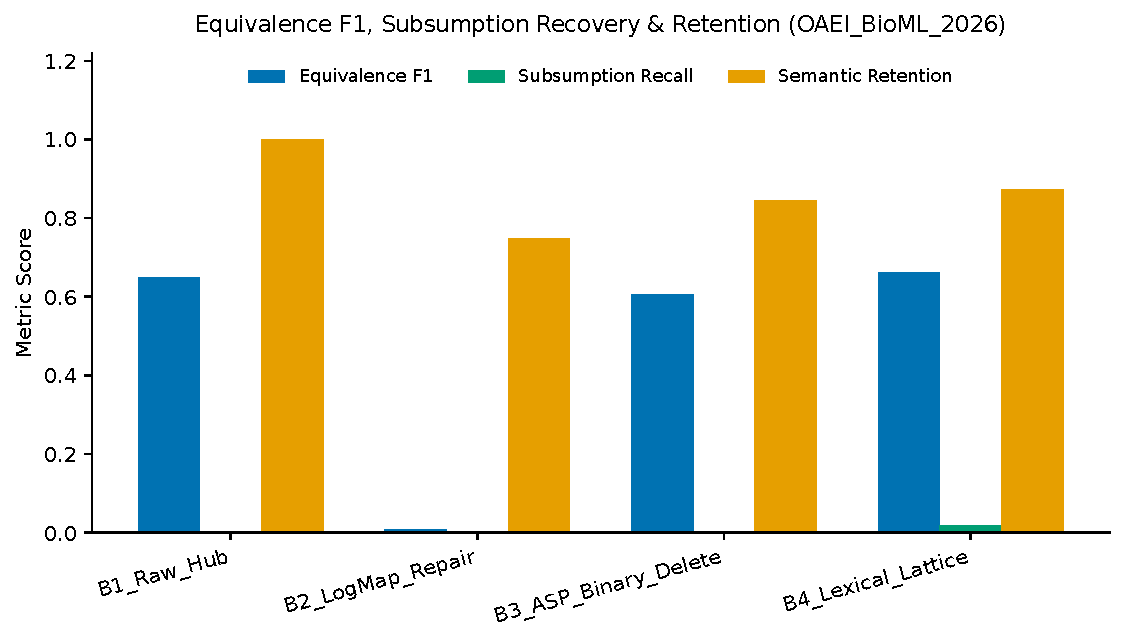
\includegraphics[width=0.86\textwidth]{../results/figures/fig2_accuracy_subsumption.pdf}
\caption{\textbf{Held-out accuracy and semantic retention on \texttt{OAEI\_BioML\_2026}.} \texttt{B4\_Lexical\_Lattice} certifies zero violations while achieving higher equivalence $F_1$ (\ClaspOAEIBioMLBLexicalLatticeEquivFone{}) than both binary hitting-set deletion (\texttt{B3}, \ClaspOAEIBioMLBASPBinaryDeleteEquivFone{}) and the uncertified raw alignment (\texttt{B1}, \ClaspOAEIBioMLBRawHubEquivFone{}).}
\label{fig:bioml_acc}
\end{figure}

\begin{figure}[t]
\centering
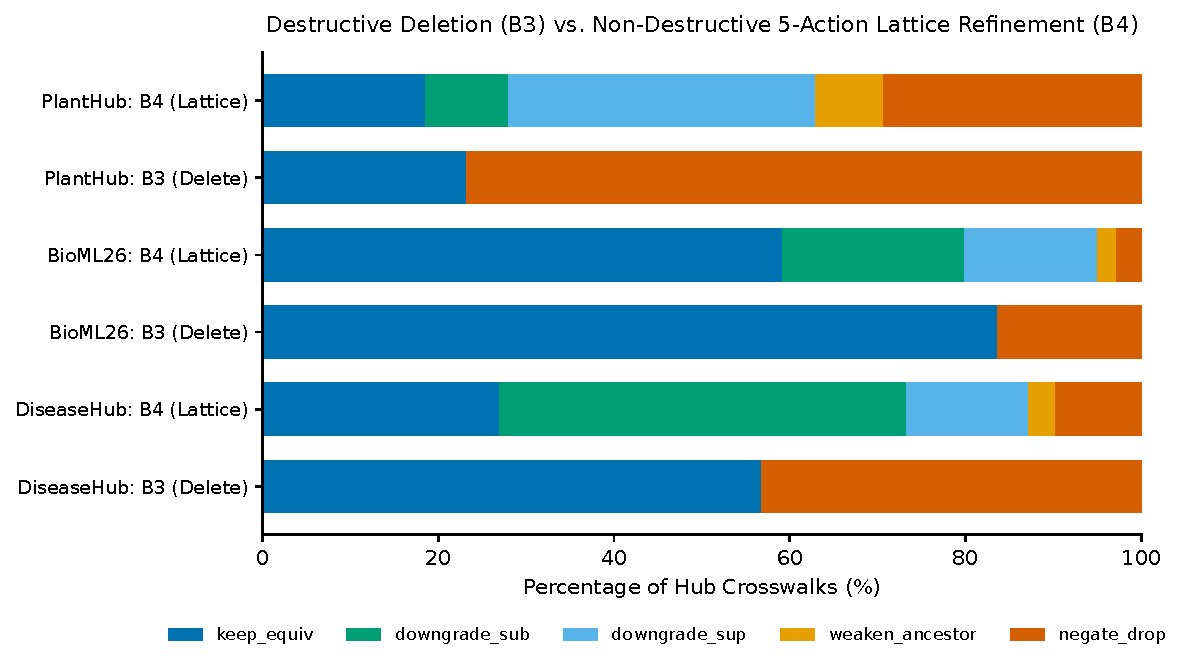
\includegraphics[width=0.90\textwidth]{../results/figures/fig3_lattice_fate_breakdown.pdf}
\caption{\textbf{Destructive deletion (\texttt{B3}) versus five-action lattice refinement (\texttt{B4}) across public hubs.} Replacing binary deletion with directional and ancestor refinements shrinks the dropped crosswalk fraction (\texttt{negate\_drop}, vermilion) from $16.4\%$ to $2.9\%$ on \texttt{OAEI\_BioML\_2026}, from $76.8\%$ to $29.4\%$ on \texttt{Plant\_Biodiv\_Hub}, and from $43.2\%$ to $9.8\%$ on \texttt{Disease\_Phenotype\_Hub}.}
\label{fig:lattice_fates}
\end{figure}

Both \texttt{B3} and \texttt{B4} achieved exact mathematical certification ($|\mathrm{Unsat}_{\Delta}| = 0$ and $|\mathrm{ConsViol}| = 0$) on every suite, but their structural impact on cross-ontology connectivity differed sharply:
\begin{itemize}[leftmargin=1.6em,itemsep=3pt,topsep=3pt]
  \item \textbf{\texttt{OAEI\_BioML\_2026}:} \texttt{B3\_ASP\_Binary\_Delete} had to discard \num{\ClaspOAEIBioMLBASPBinaryDeleteDropped} mappings, lowering held-out equivalence $F_1$ from \ClaspOAEIBioMLBRawHubEquivFone{} to \ClaspOAEIBioMLBASPBinaryDeleteEquivFone{}. \texttt{B4\_Lexical\_Lattice} discarded only \num{\ClaspOAEIBioMLBLexicalLatticeDropped} mappings ($82.5\%$ fewer deletions), converting \num{\ClaspOAEIBioMLBLexicalLatticeDowngradeSub} to $\sqsubseteq$, \num{\ClaspOAEIBioMLBLexicalLatticeDowngradeSup} to $\sqsupseteq$, and \num{\ClaspOAEIBioMLBLexicalLatticeWeakenAncestor} to ancestor subsumptions. As a result, \texttt{B4} raised held-out equivalence $F_1$ to \ClaspOAEIBioMLBLexicalLatticeEquivFone{}, surpassing both \texttt{B3} and raw \texttt{B1}, while recovering directional subsumptions (\texttt{sub\_recall} $= \ClaspOAEIBioMLBLexicalLatticeSubRecall{}$ vs.\ $0.000$ in \texttt{B1}--\texttt{B3}) and increasing semantic retention to \ClaspOAEIBioMLBLexicalLatticeRetention{} (paired contested $\Delta = +\ClaspOAEIBioMLVsBThreeMean{}$, $95\%$ bootstrap CI $[\ClaspOAEIBioMLVsBThreeLow{}, \ClaspOAEIBioMLVsBThreeHigh{}]$, two-sided Wilcoxon $q_{\mathrm{BH}} < 10^{-16}$).
  \item \textbf{\texttt{Plant\_Biodiv\_Hub}:} Because plant anatomy and environmental crosswalks intersect strict upper-ontology disjointness axioms, binary deletion (\texttt{B3}) destroyed \num{\ClaspPlantBiodivHubBASPBinaryDeleteDropped} of \num{\ClaspPlantBiodivHubMappings} mappings ($76.8\%$), leaving retention at \ClaspPlantBiodivHubBASPBinaryDeleteRetention{}. \texttt{B4\_Lexical\_Lattice} reduced deletions to \num{\ClaspPlantBiodivHubBLexicalLatticeDropped} ($-61.7\%$) by orienting \num{\ClaspPlantBiodivHubBLexicalLatticeDowngradeSub} \texttt{broadMatch}, \num{\ClaspPlantBiodivHubBLexicalLatticeDowngradeSup} \texttt{narrowMatch}, and \num{\ClaspPlantBiodivHubBLexicalLatticeWeakenAncestor} ancestor links, more than doubling semantic retention to \ClaspPlantBiodivHubBLexicalLatticeRetention{} ($\Delta = +\ClaspPlantBiodivHubVsBThreeMean{}$, $95\%$ CI $[\ClaspPlantBiodivHubVsBThreeLow{}, \ClaspPlantBiodivHubVsBThreeHigh{}]$, $q_{\mathrm{BH}} < 10^{-16}$).
  \item \textbf{\texttt{Disease\_Phenotype\_Hub}:} On the 96,273-class clinical hub, \texttt{B3} deleted \num{\ClaspDiseasePhenotypeHubBASPBinaryDeleteDropped} mappings ($43.2\%$, retention \ClaspDiseasePhenotypeHubBASPBinaryDeleteRetention{}). \texttt{B4} cut deletions by $77.3\%$ to \num{\ClaspDiseasePhenotypeHubBLexicalLatticeDropped} mappings, refining \num{\ClaspDiseasePhenotypeHubBLexicalLatticeDowngradeSub} to $\sqsubseteq$, \num{\ClaspDiseasePhenotypeHubBLexicalLatticeDowngradeSup} to $\sqsupseteq$, and \num{\ClaspDiseasePhenotypeHubBLexicalLatticeWeakenAncestor} to ancestor subsumptions, raising retention to \ClaspDiseasePhenotypeHubBLexicalLatticeRetention{} ($\Delta = +\ClaspDiseasePhenotypeHubVsBThreeMean{}$, $95\%$ CI $[\ClaspDiseasePhenotypeHubVsBThreeLow{}, \ClaspDiseasePhenotypeHubVsBThreeHigh{}]$, $q_{\mathrm{BH}} < 10^{-16}$) and unlocking \num{\ClaspDiseasePhenotypeHubBLexicalLatticeNovelCross} certified cross-ontology entailments versus \num{\ClaspDiseasePhenotypeHubBASPBinaryDeleteNovelCross} under \texttt{B3}.
\end{itemize}

We also report an instructive boundary trade-off on the synthetic \texttt{Phase0\_Toy\_Hub} control: because all 15 planted conflict traps were mislabeled equivalences whose true relation was strictly directional ($s \sqsubseteq o$ or $s \sqsubseteq \mathrm{Parent}_1(o)$), deleting all 15 traps gave \texttt{B3} a perfect equivalence $F_1$ of \ClaspPhaseToyHubBASPBinaryDeleteEquivFone{} while missing every mislabeled directional bridge (retaining only pre-existing directional inputs, \texttt{sub\_recall} $= \ClaspPhaseToyHubBASPBinaryDeleteSubRecall{}$). \texttt{B4} recovered $100\%$ of the planted directional subsumptions (\texttt{sub\_recall} $= \ClaspPhaseToyHubBLexicalLatticeSubRecall{}$, retention \ClaspPhaseToyHubBLexicalLatticeRetention{} vs.\ \ClaspPhaseToyHubBASPBinaryDeleteRetention{}, $q_{\mathrm{BH}} = 0.00096$) while converting two true equivalences in overlapping diamond cores into directional links (equivalence $F_1 = \ClaspPhaseToyHubBLexicalLatticeEquivFone{}$).

\subsection*{Biological case studies and upstream KGCL patch bundles}

Inspecting the certified KGCL patches generated by \textsc{CLASP-ONT} across the three public hubs reveals recurring ontological error patterns that binary deletion would otherwise erase (Table~\ref{tab:case_studies}; full 15-patch bundle in Supplementary Table~S2):
\begin{enumerate}[leftmargin=1.8em,itemsep=2pt,topsep=3pt]
  \item \textbf{Histological malignancy vs.\ broad neoplasm (\texttt{DOID}--\texttt{NCIT}):} High-confidence lexical matchers equate \texttt{DOID:12759} (\emph{choroid cancer}) with \texttt{NCIT:C2949} (\emph{Choroid Neoplasm}), inducing conservativity violations between benign and malignant ocular neoplasms. \textsc{CLASP-ONT} preserves the bridge as $\texttt{DOID:12759} \sqsubseteq \texttt{NCIT:C2949}$.
  \item \textbf{Phenotypic series vs.\ subtype disorder (\texttt{OMIM}--\texttt{ORDO}):} Equating \texttt{OMIM:PS115200} (\emph{Dilated cardiomyopathy} phenotypic series) with \texttt{ORDO:217604} merges heterogeneous locus-specific entries under a single clinical entity; \textsc{CLASP-ONT} refines the link to $\texttt{ORDO:217604} \sqsubseteq \texttt{OMIM:PS115200}$.
  \item \textbf{Partonomic phenotype specificity (\texttt{HP}--\texttt{MP}):} Equating \texttt{HP:0000377} (\emph{Abnormal pinna morphology}) with \texttt{MP:0002177} (\emph{abnormal outer ear morphology}) collapses external pinna defects into whole outer-ear phenotypes (which also encompass external auditory canal traits); \textsc{CLASP-ONT} certifies $\texttt{HP:0000377} \sqsubseteq \texttt{MP:0002177}$.
  \item \textbf{Taxon-specific vs.\ environmental anatomy (\texttt{PO}--\texttt{ENVO}):} Equating \texttt{PO:0009008} (\emph{plant organ}) with \texttt{ENVO:01000162} (\emph{organ}) triggers cross-kingdom disjointness cascades when animal or fungal anatomical terms enter the hub; refining to $\texttt{PO:0009008} \sqsubseteq \texttt{ENVO:01000162}$ eliminates the disjointness clash while preserving query roll-up.
\end{enumerate}

\begin{table}[t]
\centering
\caption{\textbf{Representative certified KGCL patches across oncology, rare disease, mammalian phenomics, and plant sciences.} Each patch replaces an inconsistency- or conservativity-violating \texttt{skos:exactMatch} with a certified directional subsumption.}
\label{tab:case_studies}
\footnotesize
\setlength{\tabcolsep}{4.0pt}
\resizebox{\textwidth}{!}{%
\begin{tabular}{@{}llll@{}}
\toprule
\textbf{Suite} & \textbf{Input \texttt{exactMatch} Pair} & \textbf{Certified Action} & \textbf{Exported KGCL Patch} \\
\midrule
\texttt{OAEI\_BioML\_2026} & \texttt{NCIT:C2949} $\leftrightarrow$ \texttt{DOID:12759} & \texttt{downgrade\_sup} & \texttt{create edge DOID:12759 rdfs:subClassOf NCIT:C2949} \\
\texttt{OAEI\_BioML\_2026} & \texttt{OMIM:PS115200} $\leftrightarrow$ \texttt{ORDO:217604} & \texttt{downgrade\_sup} & \texttt{create edge ORDO:217604 rdfs:subClassOf OMIM:PS115200} \\
\texttt{Disease\_Phenotype} & \texttt{HP:0000377} $\leftrightarrow$ \texttt{MP:0002177} & \texttt{downgrade\_sub} & \texttt{change ... to rdfs:subClassOf} \\
\texttt{Disease\_Phenotype} & \texttt{HP:0001547} $\leftrightarrow$ \texttt{MP:0004624} & \texttt{downgrade\_sub} & \texttt{change ... to rdfs:subClassOf} \\
\texttt{Plant\_Biodiv\_Hub} & \texttt{PO:0009008} $\leftrightarrow$ \texttt{ENVO:01000162} & \texttt{downgrade\_sub} & \texttt{change ... to rdfs:subClassOf} \\
\texttt{Plant\_Biodiv\_Hub} & \texttt{TO:0000893} $\leftrightarrow$ \texttt{FLOPO:0000093} & \texttt{downgrade\_sub} & \texttt{change ... to rdfs:subClassOf} \\
\bottomrule
\end{tabular}%
}
\end{table}

\subsection*{Laptop-scale CPU convergence and memory scaling}

A central barrier to exact multi-ontology conservativity repair has been memory blowup during justification extraction and incremental OWL reasoning. By pairing our two-tier conjunctive Horn $0\text{--}1$ BFS with indexed $\bot$-locality \textsc{QuickXplain} and unsat-core-guided \texttt{Clingo} optimization (\texttt{-{}-opt-strategy=usc,k,0,4}), \textsc{CLASP-ONT} converged monotonically to zero violations in \ClaspPlantBiodivHubBFourIters{} CEGAR iterations on \texttt{Plant\_Biodiv\_Hub}, \ClaspDiseasePhenotypeHubBFourIters{} iterations on \texttt{Disease\_Phenotype\_Hub} (\num{\ClaspDiseasePhenotypeHubTotalCores} cumulative conflict cores), and \ClaspOAEIBioMLBFourIters{} iterations on \texttt{OAEI\_BioML\_2026} (\num{\ClaspOAEIBioMLTotalCores} cumulative conflict cores; Fig.~\ref{fig:telemetry}A). Across all iterations and suites, total resident set size (Python process plus \texttt{-Xmx4G} OpenJDK~21 \texttt{ELK} subprocess and \texttt{DuckDB} out-of-core hash tables) peaked at \ClaspPlantBiodivHubPeakRssMB{}~MB on \texttt{Plant\_Biodiv\_Hub}, \ClaspOAEIBioMLPeakRssMB{}~MB on \texttt{OAEI\_BioML\_2026}, and \ClaspDiseasePhenotypeHubPeakRssMB{}~MB ($4.19$~GiB) on \texttt{Disease\_Phenotype\_Hub}, remaining well below the $6.0$~GB laptop memory ceiling (Fig.~\ref{fig:telemetry}B).

\begin{figure}[t]
\centering
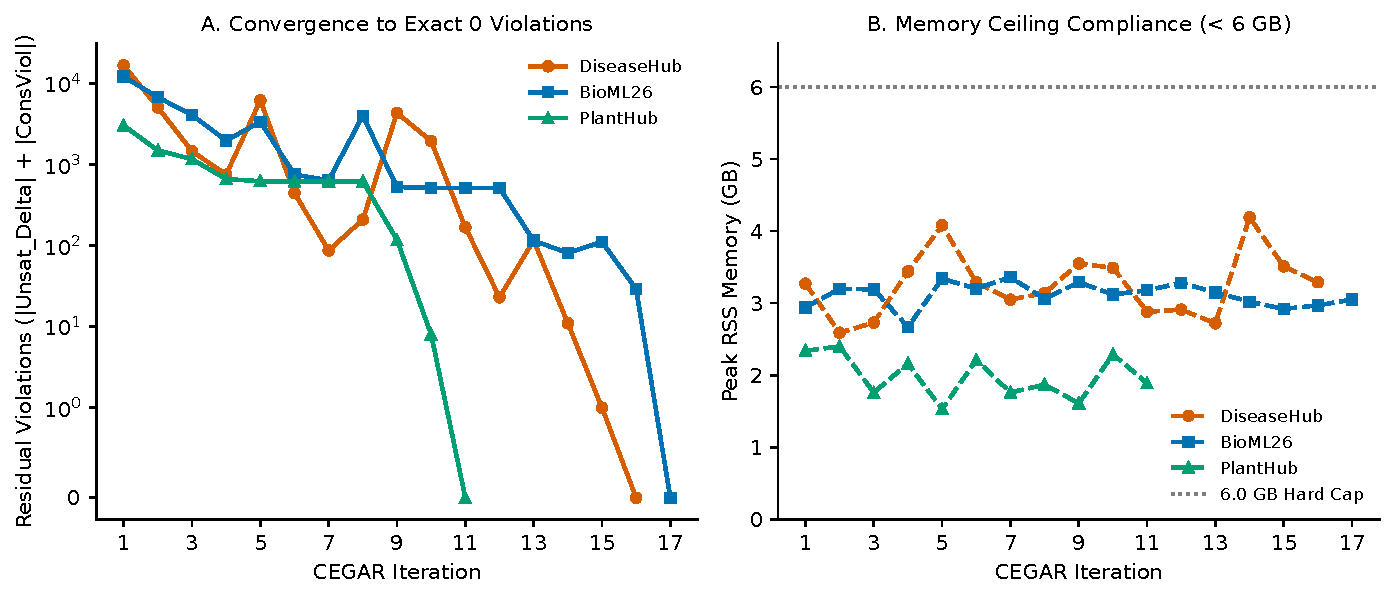
\includegraphics[width=0.96\textwidth]{../results/figures/fig5_cegar_telemetry.pdf}
\caption{\textbf{CEGAR convergence and CPU memory footprint across multi-ontology hubs.} \textbf{A.} Post-iteration residual violations ($|\mathrm{Unsat}_{\Delta}| + |\mathrm{ConsViol}|$, symmetric log scale) converge to exact zero in 11--17 iterations across all public hubs. \textbf{B.} Peak resident set size (RSS) across CEGAR iterations remains strictly below the $6.0$~GB memory cap.}
\label{fig:telemetry}
\end{figure}

\section*{Discussion}

\subsection*{Why hub-level certification matters for biological discovery and clinical systems}

Our audit demonstrates that pairwise alignment validation creates a systemic blind spot across modern life-science data infrastructure. Because OBO Foundry ontologies encode rich equivalence definitions over shared relation (\texttt{RO}) and anatomy/phenotype (\texttt{UBERON}, \texttt{HP}, \texttt{PATO}) vocabularies, asserting $s \equiv o$ between two disease or trait ontologies completes conjunctive definitions inside one ontology using existential fillers supplied by the other. On \texttt{Disease\_Phenotype\_Hub}, this cross-ontology defined-class mechanism generated thousands of single-mapping conservativity violations invisible to pure \texttt{rdfs:subClassOf} graph search, yet our conservative anonymous-witness Horn reduction captured $99.7\%$ of them in under two seconds.

Resolving these hub-level defects without mass edge deletion directly benefits four distinct communities (Table~\ref{tab:stakeholders}):
\begin{enumerate}[leftmargin=1.8em,itemsep=2pt,topsep=3pt]
  \item \textbf{Rare-disease diagnostics and cross-species phenomics:} Variant-prioritization engines rely on \texttt{HP}--\texttt{MP}--\texttt{MONDO}--\texttt{ORDO} bridges to match mouse model phenotypes against undiagnosed patient profiles. Unrepaired hubs inject \num{\ClaspDiseasePhenotypeHubRawConsViol} uncurated disease subsumptions that distort semantic similarity scores, whereas binary deletion severs $43.2\%$ of cross-ontology links; \textsc{CLASP-ONT} preserves \num{\ClaspDiseasePhenotypeHubBLexicalLatticeNovelCross} certified cross-ontology entailments ($+48{,}863$ over binary deletion) with zero contradictions.
  \item \textbf{Translational oncology and drug-target knowledge graphs:} Biopharma knowledge graphs integrating \texttt{NCIT}, \texttt{DOID}, \texttt{OMIM}, and \texttt{ORDO} require clean separation between benign neoplasms and malignant subtypes. \textsc{CLASP-ONT} prevents cohort contamination while lifting held-out \texttt{OAEI\_BioML\_2026} equivalence $F_1$ to \ClaspOAEIBioMLBLexicalLatticeEquivFone{} (versus \ClaspOAEIBioMLBLogMapRepairEquivFone{} under \texttt{LogMap} and \ClaspOAEIBioMLBASPBinaryDeleteEquivFone{} under binary deletion).
  \item \textbf{Plant genomics, crop breeding, and biodiversity portals:} Genotype-by-environment ($G \times E$) integration across \texttt{Planteome} (\texttt{PO}, \texttt{TO}), wild flora (\texttt{FLOPO}), and \texttt{ENVO} loses $76.8\%$ of its bridges under binary deletion; five-action lattice repair more than doubles retained cross-ontology utility (\ClaspPlantBiodivHubBASPBinaryDeleteRetention{} to \ClaspPlantBiodivHubBLexicalLatticeRetention{}).
  \item \textbf{OBO Foundry, \texttt{ODK}, and \texttt{Biomappings} maintainers:} Because \textsc{CLASP-ONT} requires zero GPUs and peaks below $4.3$~GB RAM, ontology release engineers can run it inside standard continuous-integration (CI) runners alongside \texttt{ROBOT} and apply its \texttt{.kgcl} output directly as reviewable pull requests.
\end{enumerate}

\begin{table}[t]
\centering
\caption{\textbf{Target communities, failure modes of current workflows, and practical value delivered by \textsc{CLASP-ONT}.}}
\label{tab:stakeholders}
\footnotesize
\setlength{\tabcolsep}{4.2pt}
\resizebox{\textwidth}{!}{%
\begin{tabular}{@{}llll@{}}
\toprule
\textbf{Target Community / Platform} & \textbf{Core Hub Ontologies} & \textbf{Failure Under Pairwise / Delete Tools} & \textbf{Value Delivered by \textsc{CLASP-ONT}} \\
\midrule
Rare-disease \& mammalian phenomics & \texttt{MONDO, ORDO, DOID, HP, MP} & \num{\ClaspDiseasePhenotypeHubRawConsViol} false subsumptions or $43.2\%$ links lost & $0$ violations; $+48{,}863$ valid cross-species links \\
Oncology \& drug-target KGs & \texttt{NCIT, DOID, OMIM, ORDO} & Benign/malignant conflation; \texttt{LogMap} $F_1 = \ClaspOAEIBioMLBLogMapRepairEquivFone{}$ & Certified $\sqsubseteq$ hierarchy; $F_1 = \ClaspOAEIBioMLBLexicalLatticeEquivFone{}$, $-82.5\%$ drops \\
Plant breeding \& $G \times E$ portals & \texttt{PO, TO, FLOPO, GO, ENVO} & $40{,}698$ unsat classes or $76.8\%$ links deleted & $2.19\times$ semantic retention at $0$ violations \\
Ontology curators (\texttt{ODK}, \texttt{Biomappings}) & Any SSSOM + OWL~2~EL hub & Pairwise QC misses $44\%\text{--}56\%$ of hub unsats & Laptop/CI gate ($<4.3$~GB RAM) + \texttt{KGCL} PRs \\
\bottomrule
\end{tabular}%
}
\end{table}

\subsection*{Scope boundaries and future extensions}

Three scope boundaries merit emphasis. First, our symbolic verifier relies on \texttt{ELK}, which is sound and complete for the polynomial OWL~2~EL profile used by large OBO Foundry ontologies (\texttt{GO}, \texttt{MONDO}, \texttt{HP}, \texttt{MP}, \texttt{PO}, \texttt{CHEBI})~\cite{kazakov2014elk,baader2005el}; ontologies that rely on universal quantification (\texttt{owl:allValuesFrom}), role inverses, or general negation require an OWL~2~DL reasoner (\texttt{HermiT} or \texttt{Konclude}) at higher computational cost. Second, while the \texttt{Clingo} CEGAR loop guarantees $100\%$ logical coherence and deductive conservativity regardless of the prior $P_{\mathrm{oracle}}(a \mid m_i)$, choosing between $s \sqsubseteq o$, $o \sqsubseteq s$, and \texttt{negate\_drop} when two ontologies have sparse text definitions, reversed tree depths, or identical homonym labels depends on the semantic prior. For instance, on \texttt{Plant\_Biodiv\_Hub}, when one direction between \texttt{PO:0025132} (\emph{plant canal}) and \texttt{ENVO:00000014} (\emph{hydrographic canal}) avoids upper-ontology disjointness axioms, the purely lexical prior (\texttt{B4}) favors directional subsumption over \texttt{negate\_drop} due to exact string overlap (Supplementary Table~S2, row~3); similarly, on \texttt{OAEI\_BioML\_2026}, \texttt{B4} achieved \ClaspOAEIBioMLBLexicalLatticeEquivFone{} equivalence $F_1$ and \ClaspOAEIBioMLBLexicalLatticeSubRecall{} held-out subsumption recall across $3{,}441$ directional reference targets, leaving clear headroom for calibrated semantic oracles. To support this extension without compromising reproducibility or data governance, \textsc{CLASP-ONT} ships a schema-validated conflict-dossier exporter ($\le 350$ tokens per contested mapping) and zero-tool, key-scrubbed sandboxed CLI runners with SHA-256 response caching (\texttt{results/oracle\_cache/}) so external semantic priors can be replayed offline in minutes without API keys. Third, strict deductive conservativity treats every novel intra-ontology subsumption as a defect; in active curation workflows where ontologies intentionally omit inferred edges, curators can inspect the exported KGCL patches to promote valid missing native edges directly into the source ontology.

\section*{Methods}

\subsection*{Formal problem specification and certification invariants}

Let $\mathcal{O} = \{O_1, \dots, O_k\}$ be $k$ OWL~2~EL ontologies with pairwise disjoint primary class signatures $\mathrm{Sig}(O_j)$ ($j \in \{1, \dots, k\}$), and let $M = \{m_1, \dots, m_n\}$ be a set of cross-ontology SSSOM correspondences $m_i = (s_i, p_i, o_i, w_i)$ with $s_i \in \mathrm{Sig}(O_a)$, $o_i \in \mathrm{Sig}(O_b)$ ($a \neq b$), predicate $p_i \in \{\texttt{skos:exactMatch}, \texttt{skos:broadMatch}, \texttt{skos:narrowMatch}\}$, and confidence $w_i \in (0, 1]$. Denote by $\mathcal{H}(\emptyset) = O_1 \cup \dots \cup O_k$ the unmapped base ontology union and by $\mathcal{H}(M) = \mathcal{H}(\emptyset) \cup \mathrm{OWL}(M)$ the merged hub. Isolating baseline entailments over $\mathcal{H}(\emptyset)$ ensures that any native unsatisfiable classes or foreign-namespace bridge axioms already embedded inside individual OBO release files are excluded from alignment-induced error counts.

\begin{definition}[Certified Multi-Ontology Hub Repair]
\label{def:certification}
Let $\Sigma_{\mathrm{all}} = \mathrm{Sig}(O_1) \cup \dots \cup \mathrm{Sig}(O_k)$, $\mathrm{Unsat}_0 = \{C \in \Sigma_{\mathrm{all}} \mid O_j \models C \sqsubseteq \bot \text{ or } \mathcal{H}(\emptyset) \models C \sqsubseteq \bot\}$, $\Sigma_{\mathrm{sat},j} = \mathrm{Sig}(O_j) \setminus \mathrm{Unsat}_0$, and $T_{0,j} = \{(A, B) \in \Sigma_{\mathrm{sat},j} \times \Sigma_{\mathrm{sat},j} \mid O_j \models A \sqsubseteq B \text{ or } \mathcal{H}(\emptyset) \models A \sqsubseteq B\}$. A refined alignment $M'$ is \emph{certified} if and only if:
\begin{align}
  \mathrm{Unsat}_{\Delta}(\mathcal{H}(M')) &= \Bigl\{ C \in \Sigma_{\mathrm{all}} \setminus \mathrm{Unsat}_0 \;\Big|\; \mathcal{H}(M') \models C \sqsubseteq \bot \Bigr\} = \emptyset, \label{eq:unsat_delta}\\
  \mathrm{ConsViol}(\mathcal{H}(M')) &= \bigcup_{j} \Bigl\{ (A, B) \in \Sigma_{\mathrm{sat},j} \times \Sigma_{\mathrm{sat},j} \;\Big|\; A \neq B,\; \mathcal{H}(M') \models A \sqsubseteq B,\; (A, B) \notin T_{0,j} \Bigr\} = \emptyset. \label{eq:consviol}
\end{align}
\end{definition}

\subsection*{The five-element subsumption refinement poset $\mathcal{L}(m_i)$}

\begin{definition}[Subsumption Refinement Poset and Minimal Conflict Core]
\label{def:poset}
For any contested correspondence $m_i = (s_i, p_i, o_i, w_i)$, its \emph{refinement poset} $(\mathcal{L}(m_i), \preceq)$ orders five candidate actions by deductive strength (Fig.~\ref{fig:poset}) with semantic retention factor $\rho : \mathcal{L}(m_i) \to [0, 1]$; a \emph{minimal conflict core} $K_r$ is an inclusion-minimal set of directional mapping literals $(m_i, \pi)$ whose conjunction with $\mathcal{H}(\emptyset)$ entails at least one element of $\mathrm{Unsat}_{\Delta} \cup \mathrm{ConsViol}$.
\end{definition}

Specifically, each contested mapping $m_i$ is assigned one action $a_i \in \mathcal{L}(m_i)$:
\begin{enumerate}[leftmargin=1.8em,itemsep=1.5pt,topsep=2pt]
  \item \texttt{keep\_equiv} ($\rho = 1.00$): retain $s_i \equiv o_i$ (or the original directional assertion if $p_i \neq \texttt{skos:exactMatch}$);
  \item \texttt{downgrade\_sub} ($\rho = 0.75$): weaken to $s_i \sqsubseteq o_i$ (\texttt{skos:broadMatch});
  \item \texttt{downgrade\_sup} ($\rho = 0.75$): weaken to $o_i \sqsubseteq s_i$ (\texttt{skos:narrowMatch});
  \item \texttt{weaken\_ancestor} ($\rho = 0.45$): weaken to $s_i \sqsubseteq \mathrm{Parent}_1(o_i)$ or $o_i \sqsubseteq \mathrm{Parent}_1(s_i)$ using the deterministic immediate named superclass in the target ontology;
  \item \texttt{negate\_drop} ($\rho = 0.00$): omit the OWL axiom from $\mathcal{H}(M')$ and emit an SSSOM negative record (\texttt{predicate\_modifier: Not}).
\end{enumerate}
If $\mathrm{Parent}_1(\cdot)$ does not exist (root class), \texttt{weaken\_ancestor} is pruned from $\mathcal{L}(m_i)$. Given semantic action probabilities $P_{\mathrm{oracle}}(a \mid m_i)$ and conflict cores $\mathcal{K}$, we maximize integer-scaled certified semantic utility:
\begin{equation}
\label{eq:asp_obj}
\max_{\mathbf{a} \in \prod_i \mathcal{L}(m_i)} \sum_{m_i \in M_{\mathrm{conflict}}} \bigl\lfloor 1000 \cdot w_i \cdot \rho(a_i) \cdot P_{\mathrm{oracle}}(a_i \mid m_i) \bigr\rfloor \quad \text{s.t.} \quad \forall K_r \in \mathcal{K},\; \neg \bigwedge_{(m_i, \pi) \in K_r} \mathrm{entails}(a_i, \pi),
\end{equation}
where $\mathrm{entails}(\texttt{keep\_equiv}, \texttt{dir\_sub})$ and $\mathrm{entails}(\texttt{keep\_equiv}, \texttt{dir\_sup})$ both hold, so any directional conflict literal $(m_i, \texttt{dir\_sub})$ automatically forbids $\texttt{keep\_equiv}$ and $\texttt{downgrade\_sub}$ while permitting $\texttt{downgrade\_sup}$ without waiting for a second CEGAR round.

\begin{figure}[t]
\centering
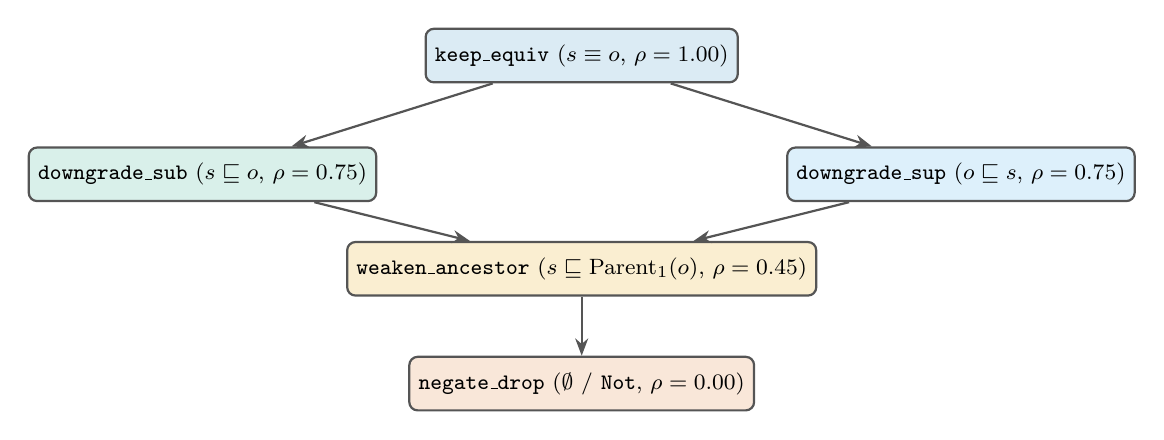
\begin{tikzpicture}[
  node distance=0.85cm and 1.6cm,
  actnode/.style={draw=oiGray, rounded corners=3pt, thick, minimum width=3.2cm, minimum height=0.68cm, align=center, font=\footnotesize},
  edgearrow/.style={-{Stealth[length=2.2mm]}, thick, color=oiGray}
]
  \node[actnode, fill=oiBlue!14] (keep) {\texttt{keep\_equiv} ($s \equiv o$, $\rho=1.00$)};
  \node[actnode, fill=oiGreen!15, below left=0.8cm and 0.6cm of keep] (sub) {\texttt{downgrade\_sub} ($s \sqsubseteq o$, $\rho=0.75$)};
  \node[actnode, fill=oiSky!20, below right=0.8cm and 0.6cm of keep] (sup) {\texttt{downgrade\_sup} ($o \sqsubseteq s$, $\rho=0.75$)};
  \node[actnode, fill=oiOrange!18, below=2.0cm of keep] (weak) {\texttt{weaken\_ancestor} ($s \sqsubseteq \mathrm{Parent}_1(o)$, $\rho=0.45$)};
  \node[actnode, fill=oiVermilion!15, below=0.75cm of weak] (drop) {\texttt{negate\_drop} ($\emptyset$ / \texttt{Not}, $\rho=0.00$)};

  \draw[edgearrow] (keep) -- (sub);
  \draw[edgearrow] (keep) -- (sup);
  \draw[edgearrow] (sub) -- (weak);
  \draw[edgearrow] (sup) -- (weak);
  \draw[edgearrow] (weak) -- (drop);
\end{tikzpicture}
\caption{\textbf{Hasse diagram of the five-element subsumption refinement poset $\mathcal{L}(m_i)$.} Directed edges denote strict deductive weakening from symmetric equivalence (\texttt{keep\_equiv}) down to negative curation (\texttt{negate\_drop}).}
\label{fig:poset}
\end{figure}

\subsection*{Stage 1: Streaming \texttt{ELK} closure and $O(|T_{\mathcal{H}}|)$ \texttt{DuckDB} conservativity diffing}

We implemented a custom headless OpenJDK~21 streaming helper (\texttt{ElkClosureRunner.java}) compiled against \texttt{ROBOT~v1.9.11}~\cite{jackson2019robot} and \texttt{ELK}~\cite{kazakov2014elk} under a hard \texttt{-Xmx4G} heap cap. For $\mathcal{H}(M^{(t)})$, \texttt{ElkClosureRunner} computes the class hierarchy once, streams $\mathrm{Unsat}$ and primary-signature transitive subsumptions $T_{\mathcal{H}}$ to Parquet via \texttt{Polars}, and evaluates Equation~\eqref{eq:consviol} in \texttt{DuckDB}~\cite{raasveldt2019duckdb}. To prevent query-planner join reordering into an $\mathcal{O}(|\mathrm{Sig}|^2)$ self-join on ontology identifiers, \texttt{conservativity.py} materializes \texttt{sig\_tbl(iri, ont\_id)} and probes \texttt{sub\_iri} and \texttt{sup\_iri} independently before executing an \texttt{ANTI JOIN} against \texttt{intra\_closure.parquet} (\texttt{memory\_limit = 3GB}), completing exact conservativity diffing over $1.4 \times 10^6$ closure pairs in $< 0.25$~s.

\subsection*{Stage 2: Two-tier conjunctive Horn $0\text{--}1$ BFS and monotonic $\bot$-locality \textsc{QuickXplain}}

Downstream shadow cascades are first condensed to root unsatisfiable classes (whose native parents are satisfiable) and generator conservativity pairs $(A, B) \in \mathrm{ConsViol}$ (where no native parent $A' \sqsupseteq A$ satisfies $(A', B) \in \mathrm{ConsViol}$ and no native child $B' \sqsubseteq B$ satisfies $(A, B') \in \mathrm{ConsViol}$).

\begin{algorithm}[t]
\caption{Two-Tier Exact Conflict Core Extraction and Max-Weight Lattice CEGAR}
\label{alg:cegar}
\small
\begin{algorithmic}[1]
\Require Ontologies $\{O_1,\dots,O_k\}$, input crosswalks $M$, priors $P_{\mathrm{oracle}}$, max iterations $T_{\max}$
\Ensure Certified actions $\mathbf{a}^*$ with $|\mathrm{Unsat}_{\Delta}(\mathcal{H}(M(\mathbf{a}^*)))| = 0$ and $|\mathrm{ConsViol}(\mathcal{H}(M(\mathbf{a}^*)))| = 0$
\State $(\mathrm{Unsat}_0, T^0, E_{\mathrm{zero}}, \mathcal{R}_{\mathrm{conj}}) \gets \textsc{PrecleanWithAnonProbes}(O_1,\dots,O_k)$ \Comment{One-way $E_\ell \sqsubseteq \texttt{urn:clasp:anon:}\ell$}
\State $(\mathrm{Unsat}_{\Delta}, \mathrm{ConsViol}) \gets \textsc{AuditHubELKDuckDB}(\mathcal{H}(M), \mathrm{Unsat}_0, T^0)$
\State $\mathcal{K} \gets \textsc{ExtractCoresTwoTier}(\mathrm{Unsat}_{\Delta}, \mathrm{ConsViol}, E_{\mathrm{zero}}, \mathcal{R}_{\mathrm{conj}}, M)$
\For{$t = 1, \dots, T_{\max}$}
  \State $\mathbf{a}^{(t)} \gets \textsc{ClingoMaxWeightUSC}(\mathcal{K}, M, P_{\mathrm{oracle}})$ \Comment{Equation~\eqref{eq:asp_obj} via \texttt{-{}-opt-strategy=usc,k,0,4}}
  \State $(\mathrm{Unsat}_{\Delta}, \mathrm{ConsViol}) \gets \textsc{AuditHubELKDuckDB}(\mathcal{H}(M(\mathbf{a}^{(t)})), \mathrm{Unsat}_0, T^0)$
  \If{$\mathrm{Unsat}_{\Delta} = \emptyset$ \textbf{and} $\mathrm{ConsViol} = \emptyset$}
    \State \Return $\mathbf{a}^{(t)}$ \Comment{Emit SHA-256 certificate, certified SSSOM, and KGCL patch file}
  \EndIf
  \State $\mathcal{K}_{\mathrm{new}} \gets \textsc{ExtractCoresTwoTier}(\mathrm{Unsat}_{\Delta}, \mathrm{ConsViol}, E_{\mathrm{zero}}, \mathcal{R}_{\mathrm{conj}}, M(\mathbf{a}^{(t)}))$
  \State $\mathcal{K} \gets \mathcal{K} \cup \mathcal{K}_{\mathrm{new}}$
\EndFor
\end{algorithmic}
\end{algorithm}

In \textbf{Tier~1} (in-memory conjunctive Horn $0\text{--}1$ BFS), during the one-time $\mathcal{H}(\emptyset)$ audit we scan all OWL~2~EL \texttt{EquivalentClasses} and \texttt{SubClassOf} axioms whose left-hand side is an \texttt{ObjectIntersectionOf}($G_1,\dots,G_m$) expression. For each anonymous operand $E_\ell$ (such as $\exists\texttt{RO:0004026}.\texttt{UBERON:0002204}$), we introduce a fresh witness class $P_\ell$ (\texttt{urn:clasp:anon:}$\ell$) with the conservative one-way inclusion $E_\ell \sqsubseteq P_\ell$ (where $P_\ell$ never occurs negatively or on any axiom left-hand side; Supplementary Proposition~S1) and record the conjunctive Horn rule $H_1 \wedge \dots \wedge H_m \Rightarrow D$ (where $H_\ell = P_\ell$ for anonymous operands and $H_\ell = G_\ell$ otherwise). Given weight-$0$ native edges $E_{\mathrm{zero}}$ (including native equivalence peers and witness edges) and weight-$1$ directional mapping half-edges $E_{\mathrm{map}}$, settled-set $0\text{--}1$ BFS with Horn counter propagation extracts minimum-mapping-cardinality derivations for both disjoint Y-forks ($\mathrm{Unsat}_{\Delta}$) and generator subsumptions ($\mathrm{ConsViol}$) in $\mathcal{O}(|V| + |E_{\mathrm{zero}}| + |E_{\mathrm{map}}| + \sum_r |G_r|)$ time per root target.

In \textbf{Tier~2} (event-driven $\bot$-locality \textsc{QuickXplain}), any residual violation involving nested role chains or filler-level mappings not explained by Tier~1 is passed to \texttt{ElkClosureRunner mus}. Using \texttt{SyntacticLocalityEvaluator(LocalityClass.BOTTOM\_BOTTOM)}~\cite{cuencagrau2008modular}, we index logical axioms once at startup; by monotonicity of syntactic $\bot$-locality (Supplementary Proposition~S2), axioms that remain $\bot$-local under the set of all object/data properties are indexed solely under their class/individual signature, avoiding hub-wide scans over ubiquitous relations such as \texttt{BFO:0000051} (\emph{has part}). Candidate mappings inside $\mathcal{M}_{\bot}(\mathcal{H}, \{c_1\})$ are ordered by BFS proximity from $c_1$, tested at progressive radii ($3 \to 25 \to 120 \to |\mathcal{M}_{\bot}|$), and minimized via non-tracing \textsc{QuickXplain} with fresh \texttt{ElkReasoner} disposal (\texttt{r.dispose()}) so heap usage never accumulates across queries.

\subsection*{Stage 3 and Stage 4: Semantic priors, sandboxed oracle protocol, and CEGAR certification}

For \texttt{B4\_Lexical\_Lattice}, \texttt{heuristic\_baseline.py} computes deterministic action priors $P_{\mathrm{B4}}(a \mid m_i)$ from normalized label/synonym token containment, character $n$-gram TF-IDF cosine similarity over \texttt{IAO:0000115} text definitions, and normalized ontology tree-depth specificity differentials ($\Delta d = d(s_i)/\bar{d}_{O_a} - d(o_i)/\bar{d}_{O_b}$), preferring $s_i \sqsubseteq o_i$ when $s_i$ lies deeper in its hierarchy or lexically specializes $o_i$. For optional multi-agent consensus runs (\texttt{C1}--\texttt{C4}), \texttt{dossier\_builder.py} serializes JSON-Schema-validated conflict dossiers ($\le 350$ tokens) and \texttt{sandbox\_cli\_runner.py} enforces five isolation invariants: scrubbing all metered \texttt{*\_API\_KEY} environment variables, executing in an empty \texttt{TemporaryDirectory} outside the repository, disabling all file/shell tools, verifying 50-item single-vs-batch parity ($\le 2\%$ disagreement), and caching SHA-256-verified responses in \texttt{results/oracle\_cache/} for temperature-scaled logarithmic opinion pooling (Supplementary Figure~S1).

In Stage~4 (\texttt{cegar\_loop.py}, Algorithm~\ref{alg:cegar}), \texttt{asp\_lattice.lp} is solved via multi-threaded Potassco \texttt{Clingo~v5.8.3}~\cite{gebser2019clingo} using unsat-core-guided optimization (\texttt{-{}-opt-strategy=usc,k,0,4}, 4 threads). Each candidate hub $\mathcal{H}(M(\mathbf{a}^{(t)}))$ is re-verified from scratch by \texttt{ELK} and \texttt{DuckDB}; no repair is accepted until Equations~\eqref{eq:unsat_delta} and~\eqref{eq:consviol} both evaluate to exact zero.

\subsection*{Evaluation datasets, baselines, and statistical analysis}

All four suites were executed with fixed random seed \texttt{20261116} on an Apple Silicon macOS workstation capped strictly at \texttt{-Xmx4G} JVM heap (full dataset provenance, SHA-256 checksums, and baseline CLI flags in Supplementary Table~S1):
\begin{itemize}[leftmargin=1.6em,itemsep=2pt,topsep=2pt]
  \item \textbf{\texttt{Phase0\_Toy\_Hub}:} 4 ontologies, \num{\ClaspPhaseToyHubClasses} classes, \num{\ClaspPhaseToyHubMappings} mappings containing 15 planted diamond, cross-kingdom disjointness, and granularity traps with exact ground-truth directional repairs.
  \item \textbf{\texttt{OAEI\_BioML\_2026}:} Checksummed \texttt{NCIT}, \texttt{DOID}, \texttt{ORDO}, and \texttt{OMIM} ontologies (\num{\ClaspOAEIBioMLClasses} classes) from Hugging Face \texttt{OAEI-ML/bio-ml} (\texttt{2026}) and Zenodo record \texttt{13119437}~\cite{he2022bioml}, evaluated on \num{\ClaspOAEIBioMLMappings} pooled candidate alignments (\texttt{mondo.sssom.tsv}, \texttt{Biomappings}, and normalized lexical candidates) against held-out \texttt{refs\_equiv} ($8{,}551$ pairs) and \texttt{refs\_subs} ($3{,}441$ directional pairs).
  \item \textbf{\texttt{Plant\_Biodiv\_Hub}:} \texttt{PO}, \texttt{TO}, \texttt{FLOPO}, \texttt{GO} (\texttt{goslim\_plant}), \texttt{CHEBI} (\texttt{chebi\_lite} plant module), and \texttt{ENVO} (\num{\ClaspPlantBiodivHubClasses} classes, \num{\ClaspPlantBiodivHubMappings} crosswalks).
  \item \textbf{\texttt{Disease\_Phenotype\_Hub}:} \texttt{MONDO}, \texttt{DOID}, \texttt{ORDO}, \texttt{HP}, and \texttt{MP} (\num{\ClaspDiseasePhenotypeHubClasses} classes, \num{\ClaspDiseasePhenotypeHubMappings} crosswalks from \texttt{mondo.sssom.tsv}, \texttt{Biomappings} CC0~\cite{hoyt2023biomappings}, and embedded cross-references).
\end{itemize}
\texttt{B2\_LogMap\_Repair} invoked standalone \texttt{LogMap~4.0} \texttt{DEBUGGER} (\texttt{-Xmx4G}) across all $\binom{k}{2}$ ontology pairs with canonical entity orientation (\texttt{entity1} $\in O_1$, \texttt{entity2} $\in O_2$). Paired differences in per-mapping retained semantic utility $w_i \rho(a_i)$ across contested mappings were tested using $10{,}000$-iteration paired bootstrap $95\%$ confidence intervals, two-sided Wilcoxon signed-rank tests, and McNemar's test, with Benjamini--Hochberg false discovery rate (FDR) control at $\alpha = 0.01$.

\section*{Declarations}

\subsection*{Ethics approval and consent to participate}
Not applicable. This study analyzes publicly available open biomedical and plant ontologies and does not involve human participants, clinical specimens, or animal experiments.

\subsection*{Consent for publication}
Not applicable.

\subsection*{Availability of data and materials}
The \textsc{CLASP-ONT} source code, Snakemake workflow, JSON schemas, certified SSSOM crosswalks, KGCL pull-request bundles, and SHA-256 dataset provenance manifests (\texttt{configs/hubs.yaml}, \texttt{docs/empirical/repro\_manifest.json}) are publicly available at \url{https://github.com/ehsanestaji/CLASP-ONT} under the OSI-approved Apache License~2.0 and will be archived on Zenodo prior to publication (\texttt{[ZENODO\_DOI\_PLACEHOLDER]}). All evaluated public datasets are openly accessible via Hugging Face (\texttt{OAEI-ML/bio-ml}), Zenodo (\texttt{10.5281/zenodo.13119437}), OBO Foundry PURLs, and \texttt{biopragmatics/biomappings} (CC0~1.0).

\subsection*{Competing interests}
[AUTHOR COMPETING INTERESTS PLACEHOLDER: e.g., The authors declare that they have no competing interests.]

\subsection*{Funding}
[AUTHOR FUNDING STATEMENT PLACEHOLDER]

\subsection*{Author Contributions}
[AUTHOR CREDIT CONTRIBUTIONS PLACEHOLDER]

\subsection*{Acknowledgments}
[AUTHOR ACKNOWLEDGMENTS AND OPTIONAL AI-ASSISTED TOOLING SIGN-OFF PLACEHOLDER; see \texttt{results/upstream\_prs/journal\_ai\_disclosure\_2026.json}.]

\bibliographystyle{unsrtnat}
\bibliography{references}

\end{document}
